 \documentclass[]{article}
\usepackage {amsmath}
\usepackage[a4paper, total={7.3in, 10.3in}]{geometry}
\usepackage{cleveref}

\usepackage[titletoc]{appendix}

\usepackage{amssymb}
%\usepackage{xcolor}
\usepackage[x11names, rgb]{xcolor}
\usepackage[utf8]{inputenc}
\usepackage{mathtools}
\usepackage{xcolor}
\usepackage{braket}
\usepackage{caption}
\usepackage{subcaption}
\usepackage{ulem}
\usepackage{cancel}
\usepackage{graphicx}
\usepackage{mathtools}
\usepackage{amsmath}  
\usepackage{amsfonts} 
\usepackage{graphicx}
\usepackage{amssymb} 
\usepackage{amsmath}
\usepackage{mathrsfs}
\usepackage{empheq}
\usepackage{amsthm}
 \usepackage{braket}
 \usepackage{amsmath}
\DeclareMathOperator\arctanh{arctanh}
\usepackage[utf8]{inputenc}
\usepackage[english]{babel}
\usepackage{graphicx}
\newtheorem{theorem}{Theorem}[section]
\newtheorem{corollary}{Corollary}[theorem]
\newtheorem{lemma}[theorem]{Lemma}
\numberwithin{equation}{section}
\newcommand{\units}[1]{\ensuremath{\,\mathrm{#1}}}
\newcommand{\braKet}[3]{#3\langle#1#3|#2#3\rangle}
\newcommand{\Tr}{\mathrm{tr}}
\newcommand{\BTr}{\mathrm{Tr}}
\newcommand{\latcfn}{\ensuremath{C}}
\usepackage{graphicx}
\newcommand{\tpm}{\ensuremath{{\,\pm\,}}}

\newcommand{\prp}{\perp}
\newcommand{\transp}{\mathsf{T}}
\newcommand{\GammaOp}{\Gamma}
\newcommand{\GammaDist}{\ensuremath{\Gamma^\text{d}}}
\newcommand{\GammaTwo}{\ensuremath{\Gamma^\text{2pt}}}
\newcommand{\GammaThr}{\ensuremath{\Gamma^\text{3pt}}}
\newcommand{\GammaDiq}{\ensuremath{\Gamma^\text{diq}}}
\newcommand{\lat}{{\text{lat}}}
\newcommand{\ren}{{\text{ren}}}
\newcommand{\unren}{{\text{unren}}}
\newcommand{\norm}{{\text{norm}}}
\newcommand{\tcdot}{{\cdot}}
\newcommand{\ldotP}{{\elll\!\cdot\!P}}

\newcommand{\myRe}{\ensuremath{\mathrm{Re}}}
\newcommand{\myIm}{\ensuremath{\mathrm{Im}}}

\newcommand{\dlangle}{{\rlap{\big\langle}\hskip 0.1em\big\langle}}
\newcommand{\drangle}{{\rlap{\big\rangle}\hskip 0.1em\big\rangle}}

\newcommand{\Wline}[1]{\ensuremath{{\mathcal{U}}[#1]}}
\newcommand{\WlineC}[1]{\ensuremath{{\mathcal{U}}{[#1]}}}
\newcommand{\WlineClat}[1]{\ensuremath{{\mathcal{U}}^\text{lat}{[#1]}}}
\newcommand{\WlineI}[2]{\ensuremath{{\mathcal{U}}#1{[#2]}}}
\newcommand{\Wlineren}[1]{\ensuremath{{\mathcal{U}}^\text{ren}[#1]}}

\newcommand{\mean}[1]{\ensuremath{\left\langle{#1}\right\rangle}}
\newcommand{\vect}[1]{\ensuremath{\boldsymbol{#1}}}
\newcommand{\vprp}[1]{\vect{#1}_{\mathrm T}}

\newcommand{\mmin}{{\text{min}}}

\newcommand{\quark}{q}
\newcommand{\nucl}[1]{{#1}}
\newcommand{\Quark}{Q}
\newcommand{\Afield}{A}

\newcommand{\MDM}{\mathcal{M}}
\newcommand{\tMDM}{\tilde{\mathcal{M}}}
\newcommand{\tAmp}{\widetilde{A}}
\newcommand{\tBmp}{\widetilde{B}}
\newcommand{\TFM}{{\hat{\mathbb{T}}}}
\newcommand{\renZ}{Z}
\newcommand{\U}{\mathcal{U}{[\mathcal{C}_{b}]}}
%\newcommand{\len}{\mathcal{L}}
\newcommand{\len}{\ell}
\newcommand{\tAmp}{\ensuremath{\widetilde{A}^{(+)}}}
\newcommand{\tBmp}{\ensuremath{\widetilde{B}^{(+)}}}
\newcommand{\Amp}{\ensuremath{A^{(+)}}}
\newcommand{\Bmp}{\ensuremath{B^{(+)}}}
\newcommand{\nplus}{\ensuremath{\bar n}}
\newcommand{\nminus}{\ensuremath{n}}


\newcommand{\TMD}{TMD\xspace}
\newcommand{\TMDs}{TMDs\xspace}

\newcommand{\sW}{\ensuremath{\text{sW}}}

\newcommand{\toddmark}[1]{\ensuremath{\Bigg[#1\Bigg]_{\text{\tiny{odd}}}}}
\newcommand{\Eu}[1]{#1}

\newcommand{\fourint}{\ensuremath{\int_\mathcal{F}}}
\newcommand{\xfourint}{\ensuremath{\int_\mathcal{M}}}


\newcommand{\conherm}{\ensuremath{(\dagger)}}
\newcommand{\conpar}{\ensuremath{(\mathrm{P})}}
\newcommand{\contime}{\ensuremath{(\mathrm{T})}}
\newcommand{\myeps}{\ensuremath{\epsilon}}

\newcommand{\xmom}[1]{{\ensuremath{[#1]}}}
\newcommand{\ktmom}[1]{{\ensuremath{(#1)}}}
\newcommand{\xktmom}[2]{{\xmom{#1}\ktmom{#2}}}

\newcommand{\bvec}{b}
\newcommand{\softf}{\mathcal{S}}
\newcommand{\mN}{m_N}
\newcommand{\nf}{n_f}


\newcommand{\sgn}{\mathrm{sgn}}
\newcommand{\nbdash}{\protect\nobreakdash-\hspace{0pt}}

\newcounter{fnnumber}
\newcounter{fnnumberamp}
\newcommand{\MSbar}{\overline{\text{MS}}}
\usepackage{makecell}
\newcommand{\kei}{k}

\newcommand{\unsub}{\text{unsubtr.}}
\newcommand{\zetahat}{{\hat \zeta}}
\newcommand{\elll}{b}
\def\epp{\epsilon^{\prime}}
\def\ep{\epsilon}
\def\vep{\varepsilon}
\def\la{\langle}
\def\ra{\rangle}
\def\ppg{\pi^+\pi^-\gamma}
\def\vp{{\bf p}}
\def\ko{K^0}
\def\kb{\bar{K^0}}
\def\ka{\kappa}
\def\al{\alpha}
\def\ab{\bar{\alpha}}
\def\be{\begin{equation}}
\def\ee{\end{equation}}
\def\bea{\begin{eqnarray}}
\def\eea{\end{eqnarray}}
\def\wh{\widehat}
\usepackage{listings}

\title{Generalized Sivers Shift TMD: $b\cdot P \neq 0$}
\author{\textbf{Hariprashad Ravikumar}} 

\date{}
\begin{document}
	\maketitle
\tableofcontents
\section{Goal: Extension to include the dependence on $x=\frac{k^{+}}{P^{+}}$}
\begin{align}
    \frac{1}{2} \bra{P,S}\ \bar{q}(0)\ \gamma^{+}\ \WlineC{\mathcal{C}_\bvec}\ q(\bvec)\ \ket{P,S}=2P^{+}\left(\textcolor{red}{\tAmp_{2B} }
		+ i \mN \epsilon_{ij} \vect{\bvec}_i \vect{S}_j\, \textcolor{red}{\tAmp_{12B} }\right)
\end{align}
Our goal is extract the Sivers-shift as a function of momentum fraction $x$
\begin{align}
   \Longrightarrow~ \langle \vect{k}_y \rangle_{TU}(\vprp{\bvec}^2,\textcolor{blue}{x},\zetahat,\eta v \tcdot P) 
	&\ \equiv\ \mN \frac{\tilde f_{1T}^{\perp(1)}(\vprp{\bvec}^2;\zetahat,\ldots,\eta v \tcdot P)}{\tilde f_1^{(0)}(\vprp{\bvec}^2;\zetahat,\ldots,\eta v \tcdot P)}\\
 &=-m_{N} \frac{\int d(b\cdot P)e^{ix(b\cdot P)} \textcolor{red}{\tAmp_{12B}(\bvec^2,\bvec \tcdot P,(\bvec \tcdot P) R(\zetahat^2)/\mN^2,-1/(\mN\zetahat)^2,\eta v \tcdot P)}}{\int d(b\cdot P)e^{ix(b\cdot P)}\textcolor{red}{\tAmp_{2B}(\bvec^2,\bvec \tcdot P,(\bvec \tcdot P) R(\zetahat^2)/\mN^2,-1/(\mN\zetahat)^2,\eta v \tcdot P)}}\\
 &=-m_{N} \frac{\int d(b\cdot P)e^{ix(b\cdot P)} \textcolor{red}{\tAmp_{12B}^{\text{Re}}(\bvec^2,\bvec \tcdot P,(\bvec \tcdot P) R(\zetahat^2)/\mN^2,-1/(\mN\zetahat)^2,\eta v \tcdot P)}}{\int d(b\cdot P)e^{ix(b\cdot P)}\textcolor{red}{\tAmp_{2B}^{\text{Re}}(\bvec^2,\bvec \tcdot P,(\bvec \tcdot P) R(\zetahat^2)/\mN^2,-1/(\mN\zetahat)^2,\eta v \tcdot P)}}.
 \end{align}
\section{Complex Amplitudes}
Let's start with \footnote{Boer, D., Gamberg, L., Musch, B., $\&$ Prokudin, A. (2011). Bessel-Weighted Asymmetries in Semi-Inclusive Deep Inelastic Scattering. ArXiv. https://doi.org/10.1007/JHEP10(2011)021}
\begin{align}
  \Phi^{[\GammaOp]}_{\text{unsub}} (\kei,P,S;v,\mu) & = \int \frac{d^4 \elll}{(2\pi)^4} \ 
  e^{i\kei \cdot \elll} 
  \underbrace{ \frac{1}{2} \bra{\nucl{P,S}}\ \bar \quark(0)\ \overbrace{ \mathcal{U}[0,\infty v]\ \mathcal{U}[\infty v,\elll] }^{\displaystyle \U} \GammaOp\ \quark(\elll)\ \ket{\nucl{P,S}} }_{\displaystyle \widetilde \Phi^{[\GammaOp]}_{\text{unsub}}(\elll,P,S;v,\mu) }\ .
  \label{eq-corrunmod}
\end{align}
The above correlator can be parameterized in terms of real-valued Lorentz-invariant amplitudes as
\begin{align}
\frac{1}{2} \Phi^{[\gamma^\mu]}_{\text{unsub}} & = P^\mu\, \Amp_2 +\kei^\mu\, \Amp_3 + \frac{1}{\mN} \epsilon^{\mu \nu \alpha \beta} P_\nu \kei_\alpha S_\beta\, \Amp_{12} + \frac{\mN^2}{(v \tcdot P)} v^\mu\, \Bmp_1 \nonumber\\
& + \frac{\mN}{v \tcdot P} \epsilon^{\mu \nu \alpha \beta} P_\nu v_\alpha S_\beta\, \Bmp_7 + \frac{ \mN}{v \tcdot P} \epsilon^{\mu \nu \alpha \beta} \kei_\nu v_\alpha S_\beta\, \Bmp_8 \nonumber\\ 
& + \frac{1}{\mN (v \tcdot P)} (\kei \tcdot S) \epsilon^{\mu \nu \alpha \beta} P_\nu \kei_\alpha v_\beta\, \Bmp_9  + \frac{\mN}{(v \tcdot P)^2} (v \tcdot S) \epsilon^{\mu \nu \alpha \beta} P_\nu \kei_\alpha v_\beta \Bmp_{10}\ . 
\label{eq-phidecomp}
\end{align}
On applying Lorentz transformations ($L$), parity transformation ($P$), time-reversal ($T$), and hermitian conjugation ($\dagger$) to the matrix elements, we find that the correlator fulfills
\begin{align}
	&(L): &\Phi^{[\GammaOp]}_{\text{unsub}}(\kei,P,S;v,\mu)  
	&= \Phi^{[\Lambda_{\slfrac{1}{2}}^{-1}\GammaOp\Lambda_{\slfrac{1}{2}}^{\phantom{-1}}]}_{\text{unsub}}(\Lambda \kei,\Lambda P, \Lambda S;\Lambda v,\mu)  \ ,\label{eq-lortrans} \displaybreak[0] \\
	&(P): &\Phi^{[\GammaOp]}_{\text{unsub}}(\kei,P,S;v,\mu)  
	&= \Phi^{[\gamma^0\GammaOp\gamma^0]}_{\text{unsub}}(\overline{\kei},\overline{P},-\overline{S};\overline{v},\mu)  \ ,\label{eq-conpar} \displaybreak[0] \\
	&(T): &\left[ \Phi^{[\GammaOp]}_{\text{unsub}}(\kei,P,S;v,\mu)  \right]^* 
	&= \Phi^{[\gamma^1 \gamma^3 \GammaOp^* \gamma^3 \gamma^1]}_{\text{unsub}}(\overline{\kei},\overline{P},\overline{S};-\overline{v},\mu)  \ , \label{eq-contime} \displaybreak[0] \\
	&(\dagger): &\left[  \Phi^{[\GammaOp]}_{\text{unsub}}(\kei,P,S;v,\mu)  \right]^* 
	&= \Phi^{[\gamma^0 \GammaOp^\dagger \gamma^0]}_{\text{unsub}}(\kei,P,S;v,\mu)  \ .\label{eq-conherm}
	\end{align}
where we denote the sign change of spatial components of a given vector $c$; that is,  $\overline{c} \equiv (c^0, -c^1, -c^2, -c^3)$. From hermiticity $(\dagger)$ follows that the $\Amp_i$ and $\Bmp_i$ in Eq.\ \eqref{eq-phidecomp} are real valued. Time reversal $(T)$ does not constrain the number of allowed structures, because it changes the sign of $v\tcdot P$. Instead, time reversal $(T)$ establishes relations between SIDIS amplitudes $A_i^{(+)}$, $B_i^{(+)}$ and Drell-Yan amplitudes $A_i^{(-)}$, $B_i^{(-)}$.
	
For any of the transformations $\mathcal{T} \in \{ L, P, T, \dagger \}$, the Eqs.\ \eqref{eq-lortrans}-\eqref{eq-conherm} are of the general form 
\begin{equation}
	\mathcal{T}_\Phi\left(\Phi(\kei,w)\right) = \Phi\left(\mathcal{T}_\kei(\kei),\mathcal{T}_w(w)\right)
\end{equation}
where we have omitted the subscript ``unsub'' and the renormalization scale $\mu$, and where the symbol $w$ summarizes all dependences on $\GammaOp$, $P$, $S$ and $v$. Here $\mathcal{T}_\Phi$ is either the identity function or complex conjugation.  The transformation rule $\mathcal{T}_\kei(\kei)$ maps onto $\Lambda \kei$, $\kei$ or $\overline{\kei}$ and thus fulfills $a \tcdot b = \mathcal{T}_\kei(a) \tcdot \mathcal{T}_\kei(b)$ for any two vectors $a$ and $b$. The Fourier-transformed correlator 
\begin{equation}
	\widetilde{\Phi}(\elll,w) =  \int d^4 \kei \ e^{-i \kei \tcdot \elll} \Phi(\kei, w)
\end{equation}
transforms according to
\begin{align}
	\mathcal{T}_\Phi\left(\widetilde{\Phi}(\elll,w) \right) & =  \int d^4 \kei \ e^{\mathcal{T}_\Phi(-i)\, \kei \tcdot \elll}\ \mathcal{T}_\Phi \left( \Phi(\kei, w) \right) \nonumber \\
	& =  \int d^4 q \ e^{\mathcal{T}_\Phi(-i)\, \mathcal{T}^{-1}_\kei(q) \tcdot \elll} \ \Phi\left(q, \mathcal{T}_w( w) \right).........................\text{(change of Variables: $\kei\rightarrow q=\mathcal{T}_\kei(\kei)$ or $\kei=\mathcal{T}^{-1}_\kei(q)$)}  \nonumber \\
	& =  \int d^4 q \ e^{\mathcal{T}_\Phi(-i)\, q \tcdot \mathcal{T}_\kei(\elll)} \ \Phi\left(q, \mathcal{T}_w( w) \right).........................(\because q \tcdot b = \mathcal{T}_\kei(q) \tcdot \mathcal{T}_\kei(b)) \nonumber \\
    & =  \int d^4 q \ e^{-iq\left(\frac{\mathcal{T}_\Phi(i)}{i}\,  \tcdot \mathcal{T}_\kei(\elll)\right)} \ \Phi\left(q, \mathcal{T}_w( w) \right)\nonumber \\
	& = \widetilde{\Phi}\left( \frac{\mathcal{T}_\Phi(i)}{i} \mathcal{T}_\kei(\elll), \mathcal{T}_w(w) \right)\, .
	\label{eq-phitildetrafo}
\end{align}
For example, $\tilde \Phi$ transforms under hermitian conjugation as
\begin{align}
	&(\dagger): &\left[ \widetilde{\Phi}^{[\GammaOp]}_{\text{unsub}}(\elll,P,S;v)  \right]^* 
	&= \widetilde{\Phi}^{[\gamma^0 \GammaOp^\dagger \gamma^0]}_{\text{unsub}}(-\elll,P,S;v)  \ .\label{eq-conhermtilde}
\end{align}
Let $f(\kei,w)$ be any of the structures preceding the invariant amplitudes in the parameterization of $\Phi$.
The structure $f(\kei,w)$ is a homogeneous function of some degree $n$ in $\kei$, i.e., $f(\alpha \kei,w) = \alpha^n f(\kei,w)$ for any number $\alpha$. 
For example, the structure $f(\kei,w) = \frac{1}{\mN (v \tcdot P)} (\kei \tcdot S) \epsilon^{\mu \nu \alpha \beta} P_\nu \kei_\alpha v_\beta$ preceding $\Bmp_9$ in Eq.\ \eqref{eq-phidecomp} has degree $n=2$.
If we define $\tilde f(\elll,w) \equiv f(- i \mN^2 \elll,w)$, then 
\begin{align}
	\mathcal{T}_\Phi\left( \tilde f(\elll, w) \right) =
	\mathcal{T}_\Phi(-i \mN^2)^n\, \mathcal{T}_\Phi\left( f( \elll, w) \right) =
	f\left( \mathcal{T}_\Phi(-i \mN^2) \mathcal{T}_\kei(\elll) , \mathcal{T}_w(w) \right) =
	\tilde f \left(  \frac{\mathcal{T}_\Phi(i)}{i} \elll, w \right)\, .
	\end{align}
This shows that $\tilde f$ transforms like $\widetilde \Phi$ in Eq.\ \eqref{eq-phitildetrafo}.
We conclude that the parameterization of $\widetilde{\Phi}$ can be found by the substitution $\kei \rightarrow -i \mN^2 \elll$ in the structures parameterizing $\Phi$, and we arrive at 
\begin{align}  \frac{1}{2}\widetilde \Phi^{[\gamma^\mu]}_{\text{unsub}}  = & P^\mu\, \tAmp_2 - i \mN^2 \elll^\mu\, \tAmp_3 - i \mN \epsilon^{\mu \nu \alpha \beta} P_\nu \elll_\alpha S_\beta\, \tAmp_{12} + \frac{\mN^2}{(v \tcdot P)} v^\mu\, \tBmp_1\nonumber\\
& + \frac{\mN}{v \tcdot P} \epsilon^{\mu \nu \alpha \beta} P_\nu v_\alpha S_\beta\, \tBmp_7  - \frac{ i \mN^3}{v \tcdot P} \epsilon^{\mu \nu \alpha \beta} \elll_\nu v_\alpha S_\beta\, \tBmp_8 \nonumber\\
& - \frac{\mN^3}{v \tcdot P} (\elll \tcdot S) \epsilon^{\mu \nu \alpha \beta} P_\nu \elll_\alpha v_\beta\, \tBmp_9  - \frac{i \mN^3}{(v \tcdot P)^2} (v \tcdot S) \epsilon^{\mu \nu \alpha \beta} P_\nu \elll_\alpha v_\beta \tBmp_{10}\ . 
\label{eq-phitildedecomp}
\end{align}

The amplitudes $\tAmp_i$ and $\tBmp_i$ introduced this way are no longer constrained to be real-valued functions. Instead, hermitian conjugation Eq.\ \eqref{eq-conhermtilde} yields the relation
\begin{equation}
	\left[ \tAmp_i(\elll^2,\elll \tcdot P, v \tcdot \elll / (v \tcdot P), \zeta^{-2},\mu^2) \right]^* = \tAmp_i(\elll^2,-\elll \tcdot P, -v \tcdot \elll / (v \tcdot P), \zeta^{-2},\mu^2)\, .\label{conditi_hermitian}
\end{equation}
In general, the amplitudes are complex,
\begin{align}
    \tilde{A}_i&=\tilde{A}^{\text{Re}}_i+i\tilde{A}^{\text{Im}}_i\\
    \tilde{B}_i&=\tilde{B}^{\text{Re}}_i+i\tilde{B}^{\text{Im}}_i
\end{align}
Because of Eq.\ \eqref{conditi_hermitian}, provided we have the amplitudes for both $\pm b$, we find
\begin{align}
    \tilde{A}^{\text{Re}}_i&=\tilde{A}^{\text{(b-even)}}_i\\
    \tilde{A}^{\text{Im}}_i&=\tilde{A}^{\text{(b-odd})}_i\\
    \tilde{B}^{\text{Re}}_i&=\tilde{B}^{\text{(b-even)}}_i\\
    \tilde{B}^{\text{Im}}_i&=\tilde{B}^{\text{(b-odd})}_i
\end{align}

\section{ Constraint $b\cdot P \neq 0$ for ($P_1=-1$)}
From
\begin{align}
    \frac{v \tcdot b}{v \tcdot P} = b \tcdot P \frac{R(\zetahat^2)}{\mN^2}
\end{align}
We have,
\begin{align}
    b_{1}|v|\left[\frac{P_{1}}{m_{N}}\left(\hat{\zeta}-\sqrt{\hat{\zeta}^2+1}\right)+\hat{\zeta}\frac{m_{N}}{P_{1}}\right]=\vec{v}_{T}\cdot\vec{b}_{T}
\end{align}
let $\vec{v}_{T}=(0,v_{3})$ and $\vec{b}_{T}=(b_{2},0)$
\begin{align}
    \mN &= 1067\text{ MeV};~~~~P_{1}=-\frac{2\pi}{L}=-\frac{2\pi}{32\times 0.114\text{ fm}}=-339.3\text{ MeV},
\end{align}
then
\begin{align}
   \Longrightarrow \left[\frac{P_{1}}{m_{N}}\left(\hat{\zeta}-\sqrt{\hat{\zeta}^2+1}\right)+\hat{\zeta}\frac{m_{N}}{P_{1}}\right]&=0\\
    \Longrightarrow \hat{\zeta} &=\sqrt{\frac{P_{1}^2}{m_{N}^{2}\left(\frac{m_{N}^{2}}{P_{1}^{2}}+2\right)}}\\
    \Aboxed{\hat{\zeta} &= \pm 0.0922238}.
\end{align}
Now,
\begin{align}
    \hat{\zeta}&=\frac{-v_{1}P_{1}}{|v|\mN}=\frac{-v_{1}P_{1}}{\left(\sqrt{v_{1}^{2}+0^{2}+v_{3}^{2}}\right)m_{N}}
\end{align}
on solving for $v_{1}$,
\begin{align}
    \Longrightarrow\Aboxed{v_{1}=\pm 0.303023~v_{3}}
\end{align}
So, we have
\begin{table}[h!]
    \centering
    \begin{tabular}{|c|c|c|}
    \hline
       $\vect{\bvec}/a$  &  $\eta v/a$ & $P\cdot aL/(2\pi)$\\
       \hline
        $(b_{1},b_{2},0)$ & $\pm n^{\prime}\cdot(v_{1},0,v_{3})$  & $(-1,0,0)$\\
        \hline
    \end{tabular}
    \caption{Parameters of Lattice QCD calculations}
    \label{tab:my_label}
\end{table}

\section{Generalized Sivers Shift}
\subsection{Deriving $\widetilde \Phi^{[\gamma^+]}$}
Let's start with the parametrization of the correlator\footnote{Musch, B. U., Hägler, P., Engelhardt, M., Negele, J. W., $\&$ Schäfer, A. (2011). Sivers and Boer-Mulders observables from lattice QCD. ArXiv. https://doi.org/10.1103/PhysRevD.85.094510},
\begin{align}
    \frac{1}{2}\widetilde \Phi^{[\gamma^\mu]}_{\unsub} & = 
		P^\mu\, \tAmp_2 - i \mN^2 \bvec^\mu\, \tAmp_3
		- i \mN \epsilon^{\mu \nu \alpha \beta} P_\nu \bvec_\alpha S_\beta\, \tAmp_{12} \nonumber \\ &
		~~+ \frac{\mN^2}{(v \tcdot P)} v^\mu\, \tBmp_1 
		+ \frac{\mN}{v \tcdot P} \epsilon^{\mu \nu \alpha \beta} P_\nu v_\alpha S_\beta\, \tBmp_7  
		- \frac{ i \mN^3}{v \tcdot P} \epsilon^{\mu \nu \alpha \beta} \bvec_\nu v_\alpha S_\beta\, \tBmp_8 \nonumber \\ &
		~~- \frac{\mN^3}{v \tcdot P} (\bvec \tcdot S) \epsilon^{\mu \nu \alpha \beta} P_\nu \bvec_\alpha v_\beta\, \tBmp_9
		- \frac{i \mN^3}{(v \tcdot P)^2} (v \tcdot S) \epsilon^{\mu \nu \alpha \beta} P_\nu \bvec_\alpha v_\beta \tBmp_{10}
\end{align}
 For the lattice calculations, it is however advantageous to start with an equivalent parametrization in which the structures explicitly depend on the staple extent $\eta$ and which is still well-defined for $v \tcdot P = 0$. Such a parametrization can be obtained from the parametrization above by replacing $v \rightarrow \eta v$ and by leaving out the factors $(v \tcdot P)^{-n}$. 
 \begin{align}
    \frac{1}{2}\widetilde \Phi^{[\gamma^\mu]}_{\unsub}=\frac{1}{2} R_{\gamma^{\mu}} E_N & =  
		P^\mu\, \tilde a_2 - i \mN^2 \bvec^\mu\, \tilde a_3
		- i \mN \epsilon^{\mu \nu \alpha \beta} P_\nu \bvec_\alpha S_\beta\, \tilde a_{12} \nonumber \\ &
		~~+ \mN^2 \eta v^\mu\, \tilde b_1 
		+ \mN \epsilon^{\mu \nu \alpha \beta} P_\nu \eta v_\alpha S_\beta\, \tilde b_7  
		-  i \mN^3 \epsilon^{\mu \nu \alpha \beta} \bvec_\nu \eta v_\alpha S_\beta\, \tilde b_8 \nonumber \\ &
		~~- \mN^3 (\bvec \tcdot S) \epsilon^{\mu \nu \alpha \beta} P_\nu \bvec_\alpha \eta v_\beta\, \tilde b_9
		-i \mN^3 (v \tcdot S) \epsilon^{\mu \nu \alpha \beta} P_\nu \bvec_\alpha \eta^2 v_\beta \tilde b_{10}
\end{align}
For $P^{\mu}=(E_N, -|\vec{P}^1|,0,0)$, $b^{\mu}=(0,b_{1},b_{2},0)$, $v^{\mu}=\pm n^{\prime}(0,v_{1},0,v_{3})$, $S^{\mu}=(0,0,0,1)$,
\begin{align}
    \frac{1}{2}\widetilde \Phi^{[\gamma^{0}]}_{\unsub} & = 
		P^0\, \tAmp_2 - \cancelto{0}{i \mN^2 \bvec^0\, \tAmp_3}
		+ i \mN \underbrace{\epsilon^{0 123}}_{1} |\vec{P}^1| \bvec_2 S_3\, \tAmp_{12} \nonumber \\ &
		~~+ \cancelto{0}{\frac{\mN^2}{(v \tcdot P)} v^0\, \tBmp_1 }
		+ \cancelto{0}{\frac{\mN}{v \tcdot P} \epsilon^{0 113} P_1 v_1 S_3\, \tBmp_7  }+ \cancelto{0}{\frac{\mN}{v \tcdot P} \epsilon^{0 133} P_1 v_3 S_3\, \tBmp_7  }
		 \nonumber \\ &
		~~- \frac{ i \mN^3}{v \tcdot P} \underbrace{\epsilon^{0 213}}_{-1} \bvec_2 v_1 S_3\, \tBmp_8 - \cancelto{0}{\frac{ i \mN^3}{v \tcdot P}\epsilon^{0 113} \bvec_1 v_1 S_3\, \tBmp_8}- \cancelto{0}{\frac{ i \mN^3}{v \tcdot P}\epsilon^{0 133} \bvec_1 v_3 S_3\, \tBmp_8}- \cancelto{0}{\frac{ i \mN^3}{v \tcdot P}\epsilon^{0 233} \bvec_2 v_3 S_3\, \tBmp_8}\nonumber \\ &
		~~+ \frac{\mN^3}{v \tcdot P} \cancelto{0}{(\bvec \tcdot S)} \underbrace{\epsilon^{0 123}}_{1} |\vec{P}_1| \bvec_2 v_3\, \tBmp_9- \cancelto{0}{\frac{\mN^3}{v \tcdot P} (\bvec \tcdot S) \epsilon^{0 121} P_1 \bvec_2 v_1\, \tBmp_9}- \cancelto{0}{\frac{\mN^3}{v \tcdot P} (\bvec \tcdot S) \epsilon^{0 113} P_1 \bvec_1 v_3\, \tBmp_9}- \cancelto{0}{\frac{\mN^3}{v \tcdot P} (\bvec \tcdot S) \epsilon^{0 111} P_1 \bvec_1 v_1\, \tBmp_9}\nonumber \\ &
		~~+ \frac{i \mN^3}{(v \tcdot P)^2} (v \tcdot S) \underbrace{\epsilon^{0 123}}_{1} |\vec{P}_1| \bvec_2 v_3 \tBmp_{10}
		- \cancelto{0}{\frac{i \mN^3}{(v \tcdot P)^2} (v \tcdot S) \epsilon^{0 121} P_1 \bvec_2 v_1 \tBmp_{10}}- \cancelto{0}{\frac{i \mN^3}{(v \tcdot P)^2} (v \tcdot S) \epsilon^{0 111} P_1 \bvec_1 v_1 \tBmp_{10}}\nonumber \\ &
		~~- \cancelto{0}{\frac{i \mN^3}{(v \tcdot P)^2} (v \tcdot S) \epsilon^{0 113} P_1 \bvec_1 v_3 \tBmp_{10}}\\
  \Aboxed{ \frac{1}{2}\widetilde \Phi^{[\gamma^{0}]}_{\unsub}& = P^0\, \tAmp_2  + i \mN  |\vec{P}^1| \bvec_2 S_3\, \tAmp_{12}+ \frac{ i \mN^3}{v \tcdot P}  \bvec_2 v_1 S_3\, \tBmp_8+ \frac{i \mN^3}{(v \tcdot P)^2} (v \tcdot S)  |P_1| \bvec_2 v_3 \tBmp_{10}}
\end{align}
and
\begin{align}
    \frac{1}{2}\widetilde \Phi^{[\gamma^{1}]}_{\unsub} & = 
		-|\vec{P}^1|\, \tAmp_2 - i \mN^2 \bvec^1\, \tAmp_3
		- i \mN \underbrace{\epsilon^{1 023}}_{-1} P_0 \bvec_2 S_3\, \tAmp_{12} \nonumber \\ &
		~~+ \frac{\mN^2}{(v \tcdot P)} v^1\, \tBmp_1 
		+ \cancelto{0}{\frac{\mN}{v \tcdot P} \epsilon^{1 013} P_0 v_1 S_3\, \tBmp_7  }+ \cancelto{0}{\frac{\mN}{v \tcdot P} \epsilon^{1 033} P_0 v_3 S_3\, \tBmp_7  }
		- \cancelto{0}{\frac{ i \mN^3}{v \tcdot P} \epsilon^{1 213} \bvec_2 v_1 S_3\, \tBmp_8}- \cancelto{0}{\frac{ i \mN^3}{v \tcdot P} \epsilon^{1 233} \bvec_2 v_3 S_3\, \tBmp_8} \nonumber \\ &
  ~~- \cancelto{0}{\frac{ i \mN^3}{v \tcdot P} \epsilon^{1 133} \bvec_1 v_3 S_3\, \tBmp_8}- \cancelto{0}{\frac{ i \mN^3}{v \tcdot P} \epsilon^{1 113} \bvec_1 v_1 S_3\, \tBmp_8}- \frac{\mN^3}{v \tcdot P} \cancelto{0}{(\bvec \tcdot S)} \underbrace{\epsilon^{1 023}}_{1} P_0 \bvec_2 v_3\, \tBmp_9- \cancelto{0}{\frac{\mN^3}{v \tcdot P} (\bvec \tcdot S) \epsilon^{1 021} P_0 \bvec_2 v_1\, \tBmp_9} \nonumber \\ &
		~~
		- \frac{i \mN^3}{(v \tcdot P)^2} (v \tcdot S) \underbrace{\epsilon^{1 023}}_{-1} P_0 \bvec_2 v_3 \tBmp_{10}- \cancelto{0}{\frac{i \mN^3}{(v \tcdot P)^2} (v \tcdot S) \epsilon^{1 021} P_0 \bvec_2 v_1 \tBmp_{10}}\\
  \Aboxed{ \frac{1}{2}\widetilde \Phi^{[\gamma^{1}]}_{\unsub} & =-|\vec{P}^1|\, \tAmp_2+ \frac{\mN^2}{(v \tcdot P)} v^1\, \tBmp_1 
		+ i \mN  P_0 \bvec_2 S_3\, \tAmp_{12}+ \frac{i \mN^3}{(v \tcdot P)^2} (v \tcdot S)  P_0 \bvec_2 v_3 \tBmp_{10}- i \mN^2 \bvec^1\, \tAmp_3}
\end{align}
for $\mu=2$
\begin{align}
    \frac{1}{2}\widetilde \Phi^{[\gamma^2]}_{\unsub} & = 
		 - i \mN^2 \bvec^2\, \tAmp_3
		- i \mN \underbrace{\epsilon^{2 0 1 3}}_{1} P_0 \bvec_1 S_3\, \tAmp_{12} \nonumber \\ &
		~~
		+ \frac{\mN}{v \tcdot P} \underbrace{\epsilon^{2 0 1 3}}_{1} P_0 v_1 S_3\, \tBmp_7  
		 \nonumber \\ &
		~~
		- \frac{i \mN^3}{(v \tcdot P)^2} (v \tcdot S) \underbrace{\epsilon^{2 0 1 3}}_{1} P_0 \bvec_1 v_3 \tBmp_{10}\\
  \Aboxed{\frac{1}{2}\widetilde \Phi^{[\gamma^2]}_{\unsub} & =- i \mN^2 \bvec^2\, \tAmp_3
		- i \mN  P_0 \bvec_1 S_3\, \tAmp_{12}+ \frac{\mN}{v \tcdot P}  P_0 v_1 S_3\, \tBmp_7- \frac{i \mN^3}{(v \tcdot P)^2} (v \tcdot S) P_0 \bvec_1 v_3 \tBmp_{10}}
\end{align}
for $\mu=3$
\begin{align}
    \frac{1}{2}\widetilde \Phi^{[\gamma^3]}_{\unsub} & = \frac{\mN^2}{(v \tcdot P)} v^3\, \tBmp_1 
		\nonumber \\ &
		~~
		- \frac{i \mN^3}{(v \tcdot P)^2} (v \tcdot S) \underbrace{\epsilon^{3 0 2 1}}_{1} P_0 \bvec_2 v_1 \tBmp_{10}\\
  \Aboxed{\frac{1}{2}\widetilde \Phi^{[\gamma^3]}_{\unsub}& = \frac{\mN^2}{(v \tcdot P)} v^3\, \tBmp_1- \frac{i \mN^3}{(v \tcdot P)^2} (v \tcdot S)  P_0 \bvec_2 v_1 \tBmp_{10}}
\end{align}
So, we have
\begin{align}
   \Aboxed{ \frac{1}{2}\widetilde \Phi^{[\gamma^{0}]}_{\unsub}& = P^0\, \tAmp_2  + i \mN  |\vec{P}^1| \bvec_2 S_3\, \tAmp_{12}+ \frac{ i \mN^3}{v \tcdot P}  \bvec_2 v_1 S_3\, \tBmp_8+ \frac{i \mN^3}{(v \tcdot P)^2} (v \tcdot S)  |P_1| \bvec_2 v_3 \tBmp_{10}}\\
   \Aboxed{ \frac{1}{2}\widetilde \Phi^{[\gamma^{1}]}_{\unsub} & =-|\vec{P}^1|\, \tAmp_2- i \mN^2 \bvec^1\, \tAmp_3+ \frac{\mN^2}{(v \tcdot P)} v^1\, \tBmp_1 
		+ i \mN  P_0 \bvec_2 S_3\, \tAmp_{12}+ \frac{i \mN^3}{(v \tcdot P)^2} (v \tcdot S)  P_0 \bvec_2 v_3 \tBmp_{10}}\\
   \Aboxed{\frac{1}{2}\widetilde \Phi^{[\gamma^2]}_{\unsub} & =- i \mN^2 \bvec^2\, \tAmp_3
		- i \mN  P_0 \bvec_1 S_3\, \tAmp_{12}+ \frac{\mN}{v \tcdot P}  P_0 v_1 S_3\, \tBmp_7- \frac{i \mN^3}{(v \tcdot P)^2} (v \tcdot S) P_0 \bvec_1 v_3 \tBmp_{10}}\\
    \Aboxed{\frac{1}{2}\widetilde \Phi^{[\gamma^3]}_{\unsub}& = \frac{\mN^2}{(v \tcdot P)} v^3\, \tBmp_1- \frac{i \mN^3}{(v \tcdot P)^2} (v \tcdot S)  P_0 \bvec_2 v_1 \tBmp_{10}}
\end{align}
\begin{align}
    \begin{pmatrix}
        \rule{0pt}{16pt} \widetilde \Phi^{[\gamma^{0}]}_{\unsub}\\
        \rule{0pt}{16pt} \widetilde \Phi^{[\gamma^{1}]}_{\unsub}\\
        \rule{0pt}{16pt} \widetilde \Phi^{[\gamma^{2}]}_{\unsub}\\
        \rule{0pt}{16pt} \widetilde \Phi^{[\gamma^{3}]}_{\unsub}
    \end{pmatrix} &=2\begin{pmatrix}
       \rule{0pt}{16pt}  P^0\, \tAmp_2  + i \mN  |\vec{P}^1| \bvec_2 S_3\, \tAmp_{12}+ \frac{ i \mN^3}{v \tcdot P}  \bvec_2 v_1 S_3\, \tBmp_8+ \frac{i \mN^3}{(v \tcdot P)^2} (v \tcdot S)  |P_1| \bvec_2 v_3 \tBmp_{10}\\
        \rule{0pt}{16pt} -|\vec{P}^1|\, \tAmp_2- i \mN^2 \bvec^1\, \tAmp_3+ \frac{\mN^2}{(v \tcdot P)} v^1\, \tBmp_1 
		+ i \mN  P_0 \bvec_2 S_3\, \tAmp_{12}+ \frac{i \mN^3}{(v \tcdot P)^2} (v \tcdot S)  P_0 \bvec_2 v_3 \tBmp_{10}\\
         \rule{0pt}{16pt} - i \mN^2 \bvec^2\, \tAmp_3
		- i \mN  P_0 \bvec_1 S_3\, \tAmp_{12}+ \frac{\mN}{v \tcdot P}  P_0 v_1 S_3\, \tBmp_7- \frac{i \mN^3}{(v \tcdot P)^2} (v \tcdot S) P_0 \bvec_1 v_3 \tBmp_{10}\\
        \rule{0pt}{16pt} \frac{\mN^2}{(v \tcdot P)} v^3\, \tBmp_1- \frac{i \mN^3}{(v \tcdot P)^2} (v \tcdot S)  P_0 \bvec_2 v_1 \tBmp_{10}
    \end{pmatrix}
\end{align}
let's write everything in upper index form,
\begin{align}
    \begin{pmatrix}
        \rule{0pt}{16pt} \widetilde \Phi^{[\gamma^{0}]}_{\unsub}\\
        \rule{0pt}{16pt} \widetilde \Phi^{[\gamma^{1}]}_{\unsub}\\
        \rule{0pt}{16pt} \widetilde \Phi^{[\gamma^{2}]}_{\unsub}\\
        \rule{0pt}{16pt} \widetilde \Phi^{[\gamma^{3}]}_{\unsub}
    \end{pmatrix} &=2\begin{pmatrix}
       \rule{0pt}{16pt}  P^0\, \tAmp_2  - i \mN  |\vec{P}^1| \bvec^2 S^3\, \tAmp_{12}- \frac{ i \mN^3}{v \tcdot P}  \bvec^2 v^1 S^3\, \tBmp_8- \frac{i \mN^3}{(v \tcdot P)^2} (v \tcdot S)  |\vec{P}^1| \bvec^2 v^3 \tBmp_{10}\\
        \rule{0pt}{16pt} -|\vec{P}^1|\, \tAmp_2- i \mN^2 \bvec^1\, \tAmp_3+ \frac{\mN^2}{(v \tcdot P)} v^1\, \tBmp_1 
		+ i \mN  P^0 \bvec^2 S^3\, \tAmp_{12}+ \frac{i \mN^3}{(v \tcdot P)^2} (v \tcdot S)  P^0 \bvec^2 v^3 \tBmp_{10}\\
         \rule{0pt}{16pt} - i \mN^2 \bvec^2\, \tAmp_3
		- i \mN  P^0 \bvec^1 S^3\, \tAmp_{12}+ \frac{\mN}{v \tcdot P}  P^0 v^1 S^3\, \tBmp_7- \frac{i \mN^3}{(v \tcdot P)^2} (v \tcdot S) P^0 \bvec^1 v^3 \tBmp_{10}\\
        \rule{0pt}{16pt} \frac{\mN^2}{(v \tcdot P)} v^3\, \tBmp_1- \frac{i \mN^3}{(v \tcdot P)^2} (v \tcdot S)  P^0 \bvec^2 v^1 \tBmp_{10}
    \end{pmatrix}
\end{align}

The relation to the upper-case amplitudes is given by
\begin{align}
	\tAmp_i\left(\bvec^2,\bvec \tcdot P,\frac{v \tcdot \bvec}{v \tcdot P}, \frac{v^2}{(v \tcdot P)^2}, \eta v \tcdot P\right) & = \tilde a_i(\bvec^2,\bvec \tcdot P, \eta v \tcdot b, (\eta v)^2, \eta v \tcdot P)    \, , \nonumber \\
	 \tBmp_i\left(\bvec^2,\bvec \tcdot P,\frac{v \tcdot \bvec}{v \tcdot P}, \frac{v^2}{(v \tcdot P)^2}, \eta v \tcdot P\right) & = (\eta v \tcdot P)^n\ \tilde b_i(\bvec^2,\bvec \tcdot P, \eta v \tcdot b, (\eta v)^2, \eta v \tcdot P)   \, ,
	\label{eq-ab}
\end{align}
In general, the amplitudes are complex,
\begin{align}
    \tilde{a}_i&=\tilde{a}^{\text{Re}}_i+i\tilde{a}^{\text{Im}}_i\\
    \tilde{b}_i&=\tilde{b}^{\text{Re}}_i+i\tilde{b}^{\text{Im}}_i
\end{align}
then
\begin{align}
    \begin{pmatrix}
        \rule{0pt}{16pt} R_{\Gamma(1)}\\
        \rule{0pt}{16pt} R_{\Gamma(2)}\\
        \rule{0pt}{16pt} R_{\Gamma(4)}\\
        \rule{0pt}{16pt} R_{\Gamma(8)}
    \end{pmatrix} = \begin{pmatrix}
        \rule{0pt}{16pt} R_{[+i\gamma^1]}\\
        \rule{0pt}{16pt} R_{[-i\gamma^2]}\\
        \rule{0pt}{16pt} R_{[+i\gamma^3]}\\
        \rule{0pt}{16pt} R_{[\gamma^0]}
    \end{pmatrix} &=2\begin{pmatrix}
        \rule{0pt}{16pt} -i\frac{|\vec{P}^1|}{E_N}\, \tilde a_2+  \frac{\mN^2}{E_N} \bvec^1\, \tilde a_3+ i\frac{\mN^2}{E_N} \eta v^1\, \tilde b_1 
		-  \mN  \bvec^2 \, \tilde a_{12}+  \mN^3  \bvec^2 \eta^2 (v^3)^2 \tilde b_{10}\\
         \rule{0pt}{16pt} -  \frac{\mN^2}{E_N} \bvec^2\, \tilde a_3
		-  \mN   \bvec^1  \tilde a_{12}-i \mN \eta  v^1  \tilde b_7+ \mN^3  \bvec^1 \eta^2 (v^3)^2 \tilde b_{10}\\
        \rule{0pt}{16pt} i\frac{\mN^2}{E_N} \eta v^3\, \tilde b_1-  \mN^3 \bvec^2 \eta^2 v^1 v^3\tilde b_{10}\\
         \rule{0pt}{16pt}   \tilde a_2  - i \mN  \frac{|\vec{P}^1|}{E_N} \bvec^2  \tilde a_{12}- \frac{ i \mN^3}{E_N}  \bvec^2 \eta v^1  \tilde b_8+ \frac{i \mN^3}{E_N}  |\vec{P}^1| \bvec^2 \eta^2 (v^3)^2 \tilde b_{10}
    \end{pmatrix}
\end{align}
\subsection{case 1: Flipping the whole $\bvec$}
let's now decompose them into real and imaginary parts for correlators, for positive $b$, we have 
\begin{align}
    \begin{pmatrix}
        \rule{0pt}{16pt} \mathfrak{Re}\{ R_{\Gamma(1)}\}^{[+b]} \\
        \rule{0pt}{16pt} \mathfrak{Im}\{ R_{\Gamma(1)}\}^{[+b]} \\
        \rule{0pt}{16pt} \mathfrak{Re}\{ R_{\Gamma(2)}\}^{[+b]} \\
        \rule{0pt}{16pt} \mathfrak{Im}\{ R_{\Gamma(2)}\}^{[+b]} \\
        \rule{0pt}{16pt} \mathfrak{Re}\{ R_{\Gamma(4)}\}^{[+b]} \\
        \rule{0pt}{16pt} \mathfrak{Im}\{ R_{\Gamma(4)}\}^{[+b]} \\
        \rule{0pt}{16pt} \mathfrak{Re}\{ R_{\Gamma(8)}\}^{[+b]} \\
        \rule{0pt}{16pt} \mathfrak{Im}\{ R_{\Gamma(8)}\}^{[+b]}
    \end{pmatrix} &= 2\begin{pmatrix}
     \rule{0pt}{16pt}   \frac{\mN^2}{E_N} \bvec^1\, \tilde a^{\text{Re}}_3-  \mN  \bvec^2 \, \tilde a^{\text{Re}}_{12}+  \mN^3  \bvec^2 \eta^2 (v^3)^2 \tilde b^{\text{Re}}_{10} +\frac{|\vec{P}^1|}{E_N}\, \tilde a^{\text{Im}}_2- \frac{\mN^2}{E_N} \eta v^1\, \tilde b^{\text{Im}}_1\\
      \rule{0pt}{16pt}  -\frac{|\vec{P}^1|}{E_N}\, \tilde a^{\text{Re}}_2+ \frac{\mN^2}{E_N} \eta v^1\, \tilde b^{\text{Re}}_1 + \frac{\mN^2}{E_N} \bvec^1\, \tilde a^{\text{Im}}_3-  \mN  \bvec^2 \, \tilde a^{\text{Im}}_{12}+  \mN^3  \bvec^2 \eta^2 (v^3)^2 \tilde b^{\text{Im}}_{10}\\
      \rule{0pt}{16pt}  -  \frac{\mN^2}{E_N} \bvec^2\, \tilde a^{\text{Re}}_3
		-  \mN   \bvec^1  \tilde a^{\text{Re}}_{12}+ \mN^3  \bvec^1 \eta^2 (v^3)^2 \tilde b^{\text{Re}}_{10}+\mN \eta v^1  \tilde b^{\text{Im}}_7 \\
      \rule{0pt}{16pt} - \mN \eta v^1  \tilde b^{\text{Re}}_7 -  \frac{\mN^2}{E_N} \bvec^2\, \tilde a^{\text{Im}}_3
		-  \mN   \bvec^1  \tilde a^{\text{Im}}_{12}+ \mN^3  \bvec^1 \eta^2 (v^3)^2 \tilde b^{\text{Im}}_{10}\\
      \rule{0pt}{16pt} -\mN^3 \bvec^2 \eta^2 v^1 v^3\tilde b^{\text{Re}}_{10}-\frac{\mN^2}{E_N} \eta v^3\, \tilde b^{\text{Im}}_1\\
      \rule{0pt}{16pt} \frac{\mN^2}{E_N} \eta v^3\, \tilde b^{\text{Re}}_1 -\mN^3 \bvec^2 \eta^2 v^1 v^3\tilde b^{\text{Im}}_{10}\\
      \rule{0pt}{16pt}  \tilde a^{\text{Re}}_2 +  \mN  \frac{|\vec{P}^1|}{E_N} \bvec^2  \tilde a^{\text{Im}}_{12}+ \frac{  \mN^3}{E_N}  \bvec^2 \eta v^1  \tilde b^{\text{Im}}_8- \frac{ \mN^3}{E_N}  |\vec{P}^1| \bvec^2 \eta^2 (v^3)^2 \tilde b^{\text{Im}}_{10}\\
      \rule{0pt}{16pt} -  \mN  \frac{|\vec{P}^1|}{E_N} \bvec^2  \tilde a^{\text{Re}}_{12}- \frac{  \mN^3}{E_N}  \bvec^2 \eta v^1  \tilde b^{\text{Re}}_8+ \frac{ \mN^3}{E_N}  |\vec{P}^1| \bvec^2 \eta^2 (v^3)^2 \tilde b^{\text{Re}}_{10}+\tilde a^{\text{Im}}_2
    \end{pmatrix}
\end{align}
and for negative $b$, (by construction $ \tilde{A}^{\text{Im}}_i=\tilde{A}^{\text{(b-odd})}_i$ and  $\tilde{B}^{\text{Im}}_i=\tilde{B}^{\text{(b-odd})}_i$) we have 
\begin{align}
    \begin{pmatrix}
        \rule{0pt}{16pt} \mathfrak{Re}\{ R_{\Gamma(1)}\}^{[-b]} \\
        \rule{0pt}{16pt} \mathfrak{Im}\{ R_{\Gamma(1)}\}^{[-b]} \\
        \rule{0pt}{16pt} \mathfrak{Re}\{ R_{\Gamma(2)}\}^{[-b]} \\
        \rule{0pt}{16pt} \mathfrak{Im}\{ R_{\Gamma(2)}\}^{[-b]} \\
        \rule{0pt}{16pt} \mathfrak{Re}\{ R_{\Gamma(4)}\}^{[-b]} \\
        \rule{0pt}{16pt} \mathfrak{Im}\{ R_{\Gamma(4)}\}^{[-b]} \\
        \rule{0pt}{16pt} \mathfrak{Re}\{ R_{\Gamma(8)}\}^{[-b]} \\
        \rule{0pt}{16pt} \mathfrak{Im}\{ R_{\Gamma(8)}\}^{[-b]}
    \end{pmatrix} &= 2\begin{pmatrix}
     \rule{0pt}{16pt}   \textcolor{red}{-}\frac{\mN^2}{E_N} \bvec^1\, \tilde a^{\text{Re}}_3\textcolor{red}{+}  \mN  \bvec^2 \, \tilde a^{\text{Re}}_{12}\textcolor{red}{-}  \mN^3  \bvec^2 \eta^2 (v^3)^2 \tilde b^{\text{Re}}_{10} \textcolor{red}{-}\frac{|\vec{P}^1|}{E_N}\, \tilde a^{\text{Im}}_2\textcolor{red}{+} \frac{\mN^2}{E_N} \eta v^1\, \tilde b^{\text{Im}}_1\\
      \rule{0pt}{16pt}  -\frac{|\vec{P}^1|}{E_N}\, \tilde a^{\text{Re}}_2+ \frac{\mN^2}{E_N} \eta v^1\, \tilde b^{\text{Re}}_1 + \frac{\mN^2}{E_N} \bvec^1\, \tilde a^{\text{Im}}_3- \mN  \bvec^2 \, \tilde a^{\text{Im}}_{12}+ \mN^3  \bvec^2 \eta^2 (v^3)^2 \tilde b^{\text{Im}}_{10}\\
      \rule{0pt}{16pt}  \textcolor{red}{+}  \frac{\mN^2}{E_N} \bvec^2\, \tilde a^{\text{Re}}_3
		\textcolor{red}{+}  \mN   \bvec^1  \tilde a^{\text{Re}}_{12}\textcolor{red}{-} \mN^3  \bvec^1 \eta^2 (v^3)^2 \tilde b^{\text{Re}}_{10}\textcolor{red}{-}\mN \eta v^1  \tilde b^{\text{Im}}_7 \\
      \rule{0pt}{16pt} - \mN \eta v^1  \tilde b^{\text{Re}}_7 - \frac{\mN^2}{E_N} \bvec^2\, \tilde a^{\text{Im}}_3
		- \mN   \bvec^1  \tilde a^{\text{Im}}_{12} +\mN^3  \bvec^1 \eta^2 (v^3)^2 \tilde b^{\text{Im}}_{10}\\
      \rule{0pt}{16pt} \textcolor{red}{+}\mN^3 \bvec^2 \eta^2 v^1 v^3\tilde b^{\text{Re}}_{10}\textcolor{red}{+}\frac{\mN^2}{E_N} \eta v^3\, \tilde b^{\text{Im}}_1\\
      \rule{0pt}{16pt} \frac{\mN^2}{E_N} \eta v^3\, \tilde b^{\text{Re}}_1 -\mN^3 \bvec^2 \eta^2 v^1 v^3\tilde b^{\text{Im}}_{10}\\
      \rule{0pt}{16pt}  \tilde a^{\text{Re}}_2 + \mN  \frac{|\vec{P}^1|}{E_N} \bvec^2  \tilde a^{\text{Im}}_{12}+ \frac{  \mN^3}{E_N}  \bvec^2 \eta v^1  \tilde b^{\text{Im}}_8- \frac{ \mN^3}{E_N}  |\vec{P}^1| \bvec^2 \eta^2 (v^3)^2 \tilde b^{\text{Im}}_{10}\\
      \rule{0pt}{16pt} \textcolor{red}{+}  \mN  \frac{|\vec{P}^1|}{E_N} \bvec^2  \tilde a^{\text{Re}}_{12}\textcolor{red}{+} \frac{  \mN^3}{E_N}  \bvec^2 \eta v^1  \tilde b^{\text{Re}}_8 \textcolor{red}{-} \frac{ \mN^3}{E_N}  |\vec{P}^1| \bvec^2 \eta^2 (v^3)^2 \tilde b^{\text{Re}}_{10}\textcolor{red}{-}\tilde a^{\text{Im}}_2
    \end{pmatrix}
\end{align}
let's now form $b-$even part as $\frac{R^{[+b]}+R^{[-b]}}{2}$,
\begin{align}
    \begin{pmatrix}
        \rule{0pt}{16pt} \mathfrak{Re}\{ R_{\Gamma(1)}\}^{[b\text{-even}]} \\
        \rule{0pt}{16pt} \mathfrak{Im}\{ R_{\Gamma(1)}\}^{[b\text{-even}]} \\
        \rule{0pt}{16pt} \mathfrak{Re}\{ R_{\Gamma(2)}\}^{[b\text{-even}]} \\
        \rule{0pt}{16pt} \mathfrak{Im}\{ R_{\Gamma(2)}\}^{[b\text{-even}]} \\
        \rule{0pt}{16pt} \mathfrak{Re}\{ R_{\Gamma(4)}\}^{[b\text{-even}]} \\
        \rule{0pt}{16pt} \mathfrak{Im}\{ R_{\Gamma(4)}\}^{[b\text{-even}]} \\
        \rule{0pt}{16pt} \mathfrak{Re}\{ R_{\Gamma(8)}\}^{[b\text{-even}]} \\
        \rule{0pt}{16pt} \mathfrak{Im}\{ R_{\Gamma(8)}\}^{[b\text{-even}]}
    \end{pmatrix} &= 2\begin{pmatrix}
     \rule{0pt}{16pt}   0\\
      \rule{0pt}{16pt}  -\frac{|\vec{P}^1|}{E_N}\, \tilde a^{\text{Re}}_2+ \frac{\mN^2}{E_N} \eta v^1\, \tilde b^{\text{Re}}_1 + \frac{\mN^2}{E_N} \bvec^1\, \tilde a^{\text{Im}}_3-  \mN  \bvec^2 \, \tilde a^{\text{Im}}_{12}+  \mN^3  \bvec^2 \eta^2 (v^3)^2 \tilde b^{\text{Im}}_{10}\\
      \rule{0pt}{16pt}  0 \\
      \rule{0pt}{16pt} - \mN \eta v^1  \tilde b^{\text{Re}}_7 -  \frac{\mN^2}{E_N} \bvec^2\, \tilde a^{\text{Im}}_3
		-  \mN   \bvec^1  \tilde a^{\text{Im}}_{12}+ \mN^3  \bvec^1 \eta^2 (v^3)^2 \tilde b^{\text{Im}}_{10}\\
      \rule{0pt}{16pt} 0\\
      \rule{0pt}{16pt} \frac{\mN^2}{E_N} \eta v^3\, \tilde b^{\text{Re}}_1 -\mN^3 \bvec^2 \eta^2 v^1 v^3\tilde b^{\text{Im}}_{10}\\
      \rule{0pt}{16pt}  \tilde a^{\text{Re}}_2 +  \mN  \frac{|\vec{P}^1|}{E_N} \bvec^2  \tilde a^{\text{Im}}_{12}+ \frac{  \mN^3}{E_N}  \bvec^2 \eta v^1  \tilde b^{\text{Im}}_8- \frac{ \mN^3}{E_N}  |\vec{P}^1| \bvec^2 \eta^2 (v^3)^2 \tilde b^{\text{Im}}_{10}\\
      \rule{0pt}{16pt} 0
    \end{pmatrix}
\end{align}
Similarly,  $b-$odd part as $\frac{R^{[+b]}-R^{[-b]}}{2}$,
\begin{align}
    \begin{pmatrix}
        \rule{0pt}{16pt} \mathfrak{Re}\{ R_{\Gamma(1)}\}^{[b\text{-odd}]} \\
        \rule{0pt}{16pt} \mathfrak{Im}\{ R_{\Gamma(1)}\}^{[b\text{-odd}]} \\
        \rule{0pt}{16pt} \mathfrak{Re}\{ R_{\Gamma(2)}\}^{[b\text{-odd}]} \\
        \rule{0pt}{16pt} \mathfrak{Im}\{ R_{\Gamma(2)}\}^{[b\text{-odd}]} \\
        \rule{0pt}{16pt} \mathfrak{Re}\{ R_{\Gamma(4)}\}^{[b\text{-odd}]} \\
        \rule{0pt}{16pt} \mathfrak{Im}\{ R_{\Gamma(4)}\}^{[b\text{-odd}]} \\
        \rule{0pt}{16pt} \mathfrak{Re}\{ R_{\Gamma(8)}\}^{[b\text{-odd}]} \\
        \rule{0pt}{16pt} \mathfrak{Im}\{ R_{\Gamma(8)}\}^{[b\text{-odd}]}
    \end{pmatrix} &= 2\begin{pmatrix}
     \rule{0pt}{16pt}   \frac{\mN^2}{E_N} \bvec^1\, \tilde a^{\text{Re}}_3-  \mN  \bvec^2 \, \tilde a^{\text{Re}}_{12}+  \mN^3  \bvec^2 \eta^2 (v^3)^2 \tilde b^{\text{Re}}_{10} +\frac{|\vec{P}^1|}{E_N}\, \tilde a^{\text{Im}}_2- \frac{\mN^2}{E_N} \eta v^1\, \tilde b^{\text{Im}}_1\\
      \rule{0pt}{16pt}  0\\
      \rule{0pt}{16pt}  -  \frac{\mN^2}{E_N} \bvec^2\, \tilde a^{\text{Re}}_3
		-  \mN   \bvec^1  \tilde a^{\text{Re}}_{12}+ \mN^3  \bvec^1 \eta^2 (v^3)^2 \tilde b^{\text{Re}}_{10}+\mN \eta v^1  \tilde b^{\text{Im}}_7 \\
      \rule{0pt}{16pt} 0\\
      \rule{0pt}{16pt} -\mN^3 \bvec^2 \eta^2 v^1 v^3\tilde b^{\text{Re}}_{10}-\frac{\mN^2}{E_N} \eta v^3\, \tilde b^{\text{Im}}_1\\
      \rule{0pt}{16pt}0\\
      \rule{0pt}{16pt} 0\\
      \rule{0pt}{16pt} -  \mN  \frac{|\vec{P}^1|}{E_N} \bvec^2  \tilde a^{\text{Re}}_{12}- \frac{  \mN^3}{E_N}  \bvec^2 \eta v^1  \tilde b^{\text{Re}}_8+ \frac{ \mN^3}{E_N}  |\vec{P}^1| \bvec^2 \eta^2 (v^3)^2 \tilde b^{\text{Re}}_{10}+\tilde a^{\text{Im}}_2
    \end{pmatrix}
\end{align}
\begin{itemize}
    \item \textcolor{red}{! The above linear equations are unsolvable as we have 8 amplitudes but 4 nontrivial equations !}
\end{itemize}

\subsection{case 2: Flipping only the $b^1=b_{L}$}
For positive $b^1$, we have 
\begin{align}
    \begin{pmatrix}
        \rule{0pt}{16pt} \mathfrak{Re}\{ R_{\Gamma(1)}\}^{[+b^1]} \\
        \rule{0pt}{16pt} \mathfrak{Im}\{ R_{\Gamma(1)}\}^{[+b^1]} \\
        \rule{0pt}{16pt} \mathfrak{Re}\{ R_{\Gamma(2)}\}^{[+b^1]} \\
        \rule{0pt}{16pt} \mathfrak{Im}\{ R_{\Gamma(2)}\}^{[+b^1]} \\
        \rule{0pt}{16pt} \mathfrak{Re}\{ R_{\Gamma(4)}\}^{[+b^1]} \\
        \rule{0pt}{16pt} \mathfrak{Im}\{ R_{\Gamma(4)}\}^{[+b^1]} \\
        \rule{0pt}{16pt} \mathfrak{Re}\{ R_{\Gamma(8)}\}^{[+b^1]} \\
        \rule{0pt}{16pt} \mathfrak{Im}\{ R_{\Gamma(8)}\}^{[+b^1]}
    \end{pmatrix} &= 2\begin{pmatrix}
     \rule{0pt}{16pt}   \frac{\mN^2}{E_N} \bvec^1\, \tilde a^{\text{Re}}_3-  \mN  \bvec^2 \, \tilde a^{\text{Re}}_{12}+  \mN^3  \bvec^2 \eta^2 (v^3)^2 \tilde b^{\text{Re}}_{10} +\frac{|\vec{P}^1|}{E_N}\, \tilde a^{\text{Im}}_2- \frac{\mN^2}{E_N} \eta v^1\, \tilde b^{\text{Im}}_1\\
      \rule{0pt}{16pt}  -\frac{|\vec{P}^1|}{E_N}\, \tilde a^{\text{Re}}_2+ \frac{\mN^2}{E_N} \eta v^1\, \tilde b^{\text{Re}}_1 + \frac{\mN^2}{E_N} \bvec^1\, \tilde a^{\text{Im}}_3-  \mN  \bvec^2 \, \tilde a^{\text{Im}}_{12}+  \mN^3  \bvec^2 \eta^2 (v^3)^2 \tilde b^{\text{Im}}_{10}\\
      \rule{0pt}{16pt}  -  \frac{\mN^2}{E_N} \bvec^2\, \tilde a^{\text{Re}}_3
		-  \mN   \bvec^1  \tilde a^{\text{Re}}_{12}+ \mN^3  \bvec^1 \eta^2 (v^3)^2 \tilde b^{\text{Re}}_{10}+\mN \eta v^1  \tilde b^{\text{Im}}_7 \\
      \rule{0pt}{16pt} - \mN \eta v^1  \tilde b^{\text{Re}}_7 -  \frac{\mN^2}{E_N} \bvec^2\, \tilde a^{\text{Im}}_3
		-  \mN   \bvec^1  \tilde a^{\text{Im}}_{12}+ \mN^3  \bvec^1 \eta^2 (v^3)^2 \tilde b^{\text{Im}}_{10}\\
      \rule{0pt}{16pt} -\mN^3 \bvec^2 \eta^2 v^1 v^3\tilde b^{\text{Re}}_{10}-\frac{\mN^2}{E_N} \eta v^3\, \tilde b^{\text{Im}}_1\\
      \rule{0pt}{16pt} \frac{\mN^2}{E_N} \eta v^3\, \tilde b^{\text{Re}}_1 -\mN^3 \bvec^2 \eta^2 v^1 v^3\tilde b^{\text{Im}}_{10}\\
      \rule{0pt}{16pt}  \tilde a^{\text{Re}}_2 +  \mN  \frac{|\vec{P}^1|}{E_N} \bvec^2  \tilde a^{\text{Im}}_{12}+ \frac{  \mN^3}{E_N}  \bvec^2 \eta v^1  \tilde b^{\text{Im}}_8- \frac{ \mN^3}{E_N}  |\vec{P}^1| \bvec^2 \eta^2 (v^3)^2 \tilde b^{\text{Im}}_{10}\\
      \rule{0pt}{16pt} -  \mN  \frac{|\vec{P}^1|}{E_N} \bvec^2  \tilde a^{\text{Re}}_{12}- \frac{  \mN^3}{E_N}  \bvec^2 \eta v^1  \tilde b^{\text{Re}}_8+ \frac{ \mN^3}{E_N}  |\vec{P}^1| \bvec^2 \eta^2 (v^3)^2 \tilde b^{\text{Re}}_{10}+\tilde a^{\text{Im}}_2
    \end{pmatrix}
\end{align}
and for negative $b^1$, by construction $\tilde{A}^{\text{Im}}_i=\tilde{A}^{\text{(b-odd})}_i=\tilde{A}^{\text{($b^1$-odd})}_i$ and  $\tilde{B}^{\text{Im}}_i=\tilde{B}^{\text{(b-odd})}_i=\tilde{B}^{\text{($b^1$-odd})}_i$ we have 
\begin{align}
    \begin{pmatrix}
        \rule{0pt}{16pt} \mathfrak{Re}\{ R_{\Gamma(1)}\}^{[-b^1]} \\
        \rule{0pt}{16pt} \mathfrak{Im}\{ R_{\Gamma(1)}\}^{[-b^1]} \\
        \rule{0pt}{16pt} \mathfrak{Re}\{ R_{\Gamma(2)}\}^{[-b^1]} \\
        \rule{0pt}{16pt} \mathfrak{Im}\{ R_{\Gamma(2)}\}^{[-b^1]} \\
        \rule{0pt}{16pt} \mathfrak{Re}\{ R_{\Gamma(4)}\}^{[-b^1]} \\
        \rule{0pt}{16pt} \mathfrak{Im}\{ R_{\Gamma(4)}\}^{[-b^1]} \\
        \rule{0pt}{16pt} \mathfrak{Re}\{ R_{\Gamma(8)}\}^{[-b^1]} \\
        \rule{0pt}{16pt} \mathfrak{Im}\{ R_{\Gamma(8)}\}^{[-b^1]}
    \end{pmatrix} &= 2\begin{pmatrix}
     \rule{0pt}{16pt}   \textcolor{red}{-}\frac{\mN^2}{E_N} \bvec^1\, \tilde a^{\text{Re}}_3-  \mN  \bvec^2 \, \tilde a^{\text{Re}}_{12}+  \mN^3  \bvec^2 \eta^2 (v^3)^2 \tilde b^{\text{Re}}_{10} \textcolor{red}{-}\frac{|\vec{P}^1|}{E_N}\, \tilde a^{\text{Im}}_2\textcolor{red}{+} \frac{\mN^2}{E_N} \eta v^1\, \tilde b^{\text{Im}}_1\\
      \rule{0pt}{16pt}  -\frac{|\vec{P}^1|}{E_N}\, \tilde a^{\text{Re}}_2+ \frac{\mN^2}{E_N} \eta v^1\, \tilde b^{\text{Re}}_1 + \frac{\mN^2}{E_N} \bvec^1\, \tilde a^{\text{Im}}_3\textcolor{red}{+} \mN  \bvec^2 \, \tilde a^{\text{Im}}_{12}\textcolor{red}{-} \mN^3  \bvec^2 \eta^2 (v^3)^2 \tilde b^{\text{Im}}_{10}\\
      \rule{0pt}{16pt}  - \frac{\mN^2}{E_N} \bvec^2\, \tilde a^{\text{Re}}_3
		\textcolor{red}{+}  \mN   \bvec^1  \tilde a^{\text{Re}}_{12}\textcolor{red}{-} \mN^3  \bvec^1 \eta^2 (v^3)^2 \tilde b^{\text{Re}}_{10}\textcolor{red}{-}\mN \eta v^1  \tilde b^{\text{Im}}_7 \\
      \rule{0pt}{16pt} - \mN \eta v^1  \tilde b^{\text{Re}}_7 \textcolor{red}{+}  \frac{\mN^2}{E_N} \bvec^2\, \tilde a^{\text{Im}}_3
		- \mN   \bvec^1  \tilde a^{\text{Im}}_{12} +\mN^3  \bvec^1 \eta^2 (v^3)^2 \tilde b^{\text{Im}}_{10}\\
      \rule{0pt}{16pt}-\mN^3 \bvec^2 \eta^2 v^1 v^3\tilde b^{\text{Re}}_{10}\textcolor{red}{+}\frac{\mN^2}{E_N} \eta v^3\, \tilde b^{\text{Im}}_1\\
      \rule{0pt}{16pt} \frac{\mN^2}{E_N} \eta v^3\, \tilde b^{\text{Re}}_1 \textcolor{red}{+} \mN^3 \bvec^2 \eta^2 v^1 v^3\tilde b^{\text{Im}}_{10}\\
      \rule{0pt}{16pt}  \tilde a^{\text{Re}}_2 \textcolor{red}{-}  \mN  \frac{|\vec{P}^1|}{E_N} \bvec^2  \tilde a^{\text{Im}}_{12}\textcolor{red}{-} \frac{  \mN^3}{E_N}  \bvec^2 \eta v^1  \tilde b^{\text{Im}}_8\textcolor{red}{+} \frac{ \mN^3}{E_N}  |\vec{P}^1| \bvec^2 \eta^2 (v^3)^2 \tilde b^{\text{Im}}_{10}\\
      \rule{0pt}{16pt} - \mN  \frac{|\vec{P}^1|}{E_N} \bvec^2  \tilde a^{\text{Re}}_{12}- \frac{  \mN^3}{E_N}  \bvec^2 \eta v^1  \tilde b^{\text{Re}}_8 + \frac{ \mN^3}{E_N}  |\vec{P}^1| \bvec^2 \eta^2 (v^3)^2 \tilde b^{\text{Re}}_{10}\textcolor{red}{-}\tilde a^{\text{Im}}_2
    \end{pmatrix}
\end{align}
let's now form $b-$even part as $\frac{R^{[+b]}+R^{[-b]}}{2}$,
\begin{align}
    \begin{pmatrix}
        \rule{0pt}{16pt} \mathfrak{Re}\{ R_{\Gamma(1)}\}^{[b^{1}\text{-even}]} \\
        \rule{0pt}{16pt} \mathfrak{Im}\{ R_{\Gamma(1)}\}^{[b^{1}\text{-even}]} \\
        \rule{0pt}{16pt} \mathfrak{Re}\{ R_{\Gamma(2)}\}^{[b^{1}\text{-even}]} \\
        \rule{0pt}{16pt} \mathfrak{Im}\{ R_{\Gamma(2)}\}^{[b^{1}\text{-even}]} \\
        \rule{0pt}{16pt} \mathfrak{Re}\{ R_{\Gamma(4)}\}^{[b^{1}\text{-even}]} \\
        \rule{0pt}{16pt} \mathfrak{Im}\{ R_{\Gamma(4)}\}^{[b^{1}\text{-even}]} \\
        \rule{0pt}{16pt} \mathfrak{Re}\{ R_{\Gamma(8)}\}^{[b^{1}\text{-even}]} \\
        \rule{0pt}{16pt} \mathfrak{Im}\{ R_{\Gamma(8)}\}^{[b^{1}\text{-even}]}
    \end{pmatrix} &= 2\begin{pmatrix}
     \rule{0pt}{16pt}  -  \mN  \bvec^2 \, \tilde a^{\text{Re}}_{12}+  \mN^3  \bvec^2 \eta^2 (v^3)^2 \tilde b^{\text{Re}}_{10} \\
      \rule{0pt}{16pt}  -\frac{|\vec{P}^1|}{E_N}\, \tilde a^{\text{Re}}_2+ \frac{\mN^2}{E_N} \eta v^1\, \tilde b^{\text{Re}}_1 + \frac{\mN^2}{E_N} \bvec^1\, \tilde a^{\text{Im}}_3\\
      \rule{0pt}{16pt}  -  \frac{\mN^2}{E_N} \bvec^2\, \tilde a^{\text{Re}}_3
		\\
      \rule{0pt}{16pt} - \mN \eta v^1  \tilde b^{\text{Re}}_7
		-  \mN   \bvec^1  \tilde a^{\text{Im}}_{12}+ \mN^3  \bvec^1 \eta^2 (v^3)^2 \tilde b^{\text{Im}}_{10}\\
      \rule{0pt}{16pt} -\mN^3 \bvec^2 \eta^2 v^1 v^3\tilde b^{\text{Re}}_{10}\\
      \rule{0pt}{16pt} \frac{\mN^2}{E_N} \eta v^3\, \tilde b^{\text{Re}}_1 \\
      \rule{0pt}{16pt}  \tilde a^{\text{Re}}_2\\
      \rule{0pt}{16pt} -  \mN  \frac{|\vec{P}^1|}{E_N} \bvec^2  \tilde a^{\text{Re}}_{12}- \frac{  \mN^3}{E_N}  \bvec^2 \eta v^1  \tilde b^{\text{Re}}_8+ \frac{ \mN^3}{E_N}  |\vec{P}^1| \bvec^2 \eta^2 (v^3)^2 \tilde b^{\text{Re}}_{10}
    \end{pmatrix}
\end{align}
Similarly,  $b-$odd part as $\frac{R^{[+b]}-R^{[-b]}}{2}$,
\begin{align}
    \begin{pmatrix}
        \rule{0pt}{16pt} \mathfrak{Re}\{ R_{\Gamma(1)}\}^{[b^{1}\text{-odd}]} \\
        \rule{0pt}{16pt} \mathfrak{Im}\{ R_{\Gamma(1)}\}^{[b^{1}\text{-odd}]} \\
        \rule{0pt}{16pt} \mathfrak{Re}\{ R_{\Gamma(2)}\}^{[b^{1}\text{-odd}]} \\
        \rule{0pt}{16pt} \mathfrak{Im}\{ R_{\Gamma(2)}\}^{[b^{1}\text{-odd}]} \\
        \rule{0pt}{16pt} \mathfrak{Re}\{ R_{\Gamma(4)}\}^{[b^{1}\text{-odd}]} \\
        \rule{0pt}{16pt} \mathfrak{Im}\{ R_{\Gamma(4)}\}^{[b^{1}\text{-odd}]} \\
        \rule{0pt}{16pt} \mathfrak{Re}\{ R_{\Gamma(8)}\}^{[b^{1}\text{-odd}]} \\
        \rule{0pt}{16pt} \mathfrak{Im}\{ R_{\Gamma(8)}\}^{[b^{1}\text{-odd}]}
    \end{pmatrix} &= 2\begin{pmatrix}
     \rule{0pt}{16pt}   \frac{\mN^2}{E_N} \bvec^1\, \tilde a^{\text{Re}}_3+\frac{|\vec{P}^1|}{E_N}\, \tilde a^{\text{Im}}_2- \frac{\mN^2}{E_N} \eta v^1\, \tilde b^{\text{Im}}_1\\
      \rule{0pt}{16pt}  -  \mN  \bvec^2 \, \tilde a^{\text{Im}}_{12}+  \mN^3  \bvec^2 \eta^2 (v^3)^2 \tilde b^{\text{Im}}_{10}\\
      \rule{0pt}{16pt}  
		-  \mN   \bvec^1  \tilde a^{\text{Re}}_{12}+ \mN^3  \bvec^1 \eta^2 (v^3)^2 \tilde b^{\text{Re}}_{10}+\mN \eta v^1  \tilde b^{\text{Im}}_7 \\
      \rule{0pt}{16pt}  -  \frac{\mN^2}{E_N} \bvec^2\, \tilde a^{\text{Im}}_3\\
      \rule{0pt}{16pt} -\frac{\mN^2}{E_N} \eta v^3\, \tilde b^{\text{Im}}_1\\
      \rule{0pt}{16pt}  -\mN^3 \bvec^2 \eta^2 v^1 v^3\tilde b^{\text{Im}}_{10}\\
      \rule{0pt}{16pt}    \mN  \frac{|\vec{P}^1|}{E_N} \bvec^2  \tilde a^{\text{Im}}_{12}+ \frac{  \mN^3}{E_N}  \bvec^2 \eta v^1  \tilde b^{\text{Im}}_8- \frac{ \mN^3}{E_N}  |\vec{P}^1| \bvec^2 \eta^2 (v^3)^2 \tilde b^{\text{Im}}_{10}\\
      \rule{0pt}{16pt} \tilde a^{\text{Im}}_2
    \end{pmatrix}
\end{align}
to form Sivers shift all that we need are real and imaginart parts of $\tilde a_2$, $\tilde b_1$, $\tilde a_{12}$ and, $\tilde b_8$, let's extract the amplitudes for both real and imaginary parts of amplitude. For real part
\begin{align}
    \Aboxed{\tilde a^{\text{Re}}_2 = & \frac{1}{2}\mathfrak{Re}\{ R_{\Gamma(8)}\}^{[b^{1}\text{-even}]} }\\
    \Aboxed{\tilde b^{\text{Re}}_1 = & \frac{E_{N}}{2\mN^2 \eta v^3} \mathfrak{Im}\{ R_{\Gamma(4)}\}^{[b^{1}\text{-even}]}}
\end{align}
also
\begin{align}
   \Aboxed{\tilde a^{\text{Re}}_{12}=&\frac{-1}{2\mN  \bvec^2}\left[\mathfrak{Re}\{ R_{\Gamma(1)}\}^{[b^{1}\text{-even}]}+\frac{v^3}{v^1}\mathfrak{Re}\{ R_{\Gamma(4)}\}^{[b^{1}\text{-even}]}\right]}
\end{align}
\begin{align}
    \Aboxed{\tilde b^{\text{Re}}_8=&\frac{-E_N}{ 2\mN^3 \bvec^2 \eta v^1 }\left[\mathfrak{Im}\{ R_{\Gamma(8)}\}^{[b^{1}\text{-even}]}+\frac{|\vec{P}^1|v^3}{E_N v^1}\mathfrak{Re}\{ R_{\Gamma(4)}\}^{[b^{1}\text{-even}]}+ 2\mN  \frac{|\vec{P}^1|}{E_N} \bvec^2  \tilde a^{\text{Re}}_{12}\right]}
\end{align}
Similarly,  
\begin{align}
    \Aboxed{\tilde a^{\text{Im}}_2 = & \frac{1}{2}\mathfrak{Im}\{ R_{\Gamma(8)}\}^{[b^{1}\text{-odd}]} }\\
    \Aboxed{\tilde b^{\text{Im}}_1 = & \frac{-E_{N}}{2\mN^2 \eta v^3} \mathfrak{Re}\{ R_{\Gamma(4)}\}^{[b^{1}\text{-odd}]}}
\end{align}
also
\begin{align}
   \Aboxed{\tilde a^{\text{Im}}_{12}=&\frac{-1}{2\mN  \bvec^2}\left[\mathfrak{Im}\{ R_{\Gamma(1)}\}^{[b^{1}\text{-odd}]}+\frac{v^3}{v^1}\mathfrak{Im}\{ R_{\Gamma(4)}\}^{[b^{1}\text{-odd}]}\right]}
\end{align}
\begin{align}
    \Aboxed{\tilde b^{\text{Im}}_8=&\frac{E_N}{ 2\mN^3 \bvec^2 \eta v^1 }\left[\mathfrak{Re}\{ R_{\Gamma(8)}\}^{[b^{1}\text{-odd}]}-\frac{|\vec{P}^1|v^3}{E_N v^1}\mathfrak{Im}\{ R_{\Gamma(4)}\}^{[b^{1}\text{-odd}]}- 2\mN  \frac{|\vec{P}^1|}{E_N} \bvec^2  \tilde a^{\text{Im}}_{12}\right]}
\end{align}
With the dictionary 
\begin{align}
	\tAmp_i & = \tilde a_i \\
	 \tBmp_i & = (\eta v \tcdot P)^n\ \tilde b_i
\end{align}
We get,
\begin{align}
    \Aboxed{\tAmp^{\text{Re}}_2 = & \frac{1}{2}\mathfrak{Re}\{ R_{\Gamma(8)}\}^{[b^{1}\text{-even}]} }\\
    \Aboxed{\tBmp^{\text{Re}}_1 = & \frac{E_{N}|P^1|v^1}{2\mN^2  v^3} \mathfrak{Im}\{ R_{\Gamma(4)}\}^{[b^{1}\text{-even}]}}\\
    \Aboxed{\tAmp^{\text{Re}}_{12}=&\frac{-1}{2\mN  \bvec^2}\left[\mathfrak{Re}\{ R_{\Gamma(1)}\}^{[b^{1}\text{-even}]}+\frac{v^3}{v^1}\mathfrak{Re}\{ R_{\Gamma(4)}\}^{[b^{1}\text{-even}]}\right]}\\
    \Aboxed{\tBmp^{\text{Re}}_8=&\frac{-E_N |P^1|}{ 2\mN^3 \bvec^2 }\left[\mathfrak{Im}\{ R_{\Gamma(8)}\}^{[b^{1}\text{-even}]}+\frac{|\vec{P}^1|v^3}{E_N v^1}\mathfrak{Re}\{ R_{\Gamma(4)}\}^{[b^{1}\text{-even}]}+ 2\mN  \frac{|\vec{P}^1|}{E_N} \bvec^2  \tAmp^{\text{Re}}_{12}\right]}
\end{align}
\begin{align}
    \Aboxed{\tAmp^{\text{Im}}_2 = & \frac{1}{2}\mathfrak{Im}\{ R_{\Gamma(8)}\}^{[b^{1}\text{-odd}]} }\\
    \Aboxed{\tBmp^{\text{Im}}_1 = & \frac{-E_{N}|P^1|v^1}{2\mN^2 \eta v^3} \mathfrak{Re}\{ R_{\Gamma(4)}\}^{[b^{1}\text{-odd}]}}\\
    \Aboxed{\tAmp^{\text{Im}}_{12}=&\frac{-1}{2\mN  \bvec^2}\left[\mathfrak{Im}\{ R_{\Gamma(1)}\}^{[b^{1}\text{-odd}]}+\frac{v^3}{v^1}\mathfrak{Im}\{ R_{\Gamma(4)}\}^{[b^{1}\text{-odd}]}\right]}\\
     \Aboxed{\tBmp^{\text{Im}}_8=&\frac{E_N|P^1|}{ 2\mN^3 \bvec^2  }\left[\mathfrak{Re}\{ R_{\Gamma(8)}\}^{[b^{1}\text{-odd}]}-\frac{|\vec{P}^1|v^3}{E_N v^1}\mathfrak{Im}\{ R_{\Gamma(4)}\}^{[b^{1}\text{-odd}]}- 2\mN  \frac{|\vec{P}^1|}{E_N} \bvec^2  \tAmp^{\text{Im}}_{12}\right]}
\end{align}
To form Sivers shift, we use
\begin{align}
    \Aboxed{\tAmp_{2B}  & \ \equiv\  \tAmp_2 + R(\zetahat^2) \tBmp_1}\\
    \Aboxed{\tAmp_{12B}  & \ \equiv\  \tAmp_{12} - R(\zetahat^2) \tBmp_8}
\end{align}
where,
\begin{align}
    \Aboxed{R(\zetahat^2) \equiv 1- \sqrt{1 + \hat \zeta^{-2}}}
\end{align}

\section{Lattice calculations ($\tAmp_{2B}$ for $\eta=0$)}
\subsubsection{$\tAmp^{\text{Re}}_{2B}=\tAmp^{\text{(b-even)}}_{2B}$}
\begin{figure}[h!]
    \centering
    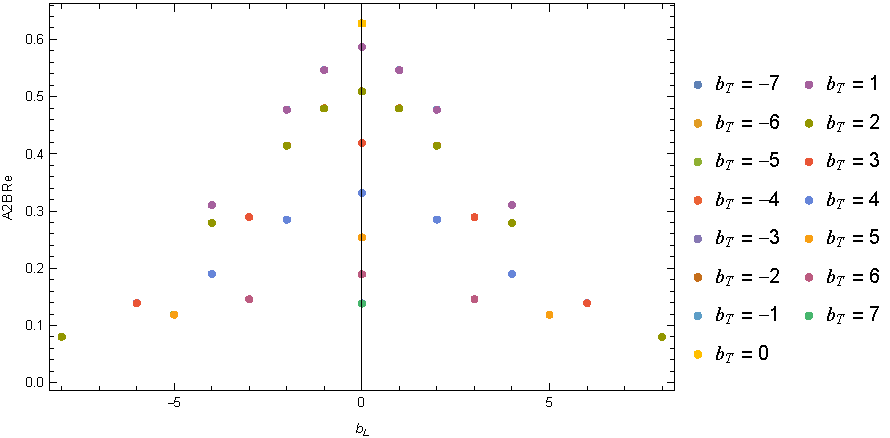
\includegraphics[width=0.45\linewidth]{bLbT_A2B_b_even_P1_-1_eta_0.pdf}
    \caption{Plot of  $\tAmp^{\text{Re}}_{2B}=\tAmp^{\text{(b-even)}}_{2B}$ for different $b_{L}$ and $b_{T}$  ($P_{1} = -1$ , $\eta=0$)}
\end{figure}

And below is the plot of $\tAmp^{\text{Re}}_{2B}=\tAmp^{\text{(b-even)}}_{2B}$ for different Lorentz invariant $P\cdot b$ and $(b)^2$,
\begin{figure}[h!]
     \centering
     \begin{subfigure}[b]{0.45\textwidth}
         \centering
         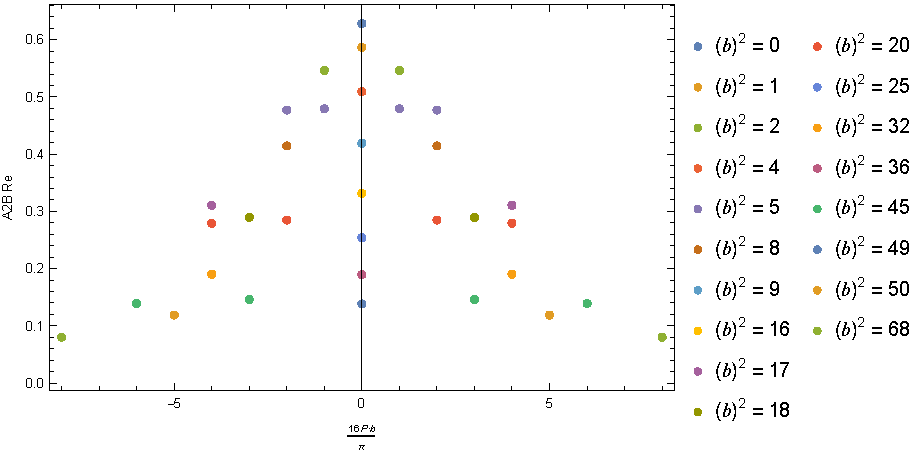
\includegraphics[width=\textwidth]{bP_A2B_b_even_P1_-1_eta_0.pdf}
     \end{subfigure}
     \begin{subfigure}[b]{0.45\textwidth}
         \centering
         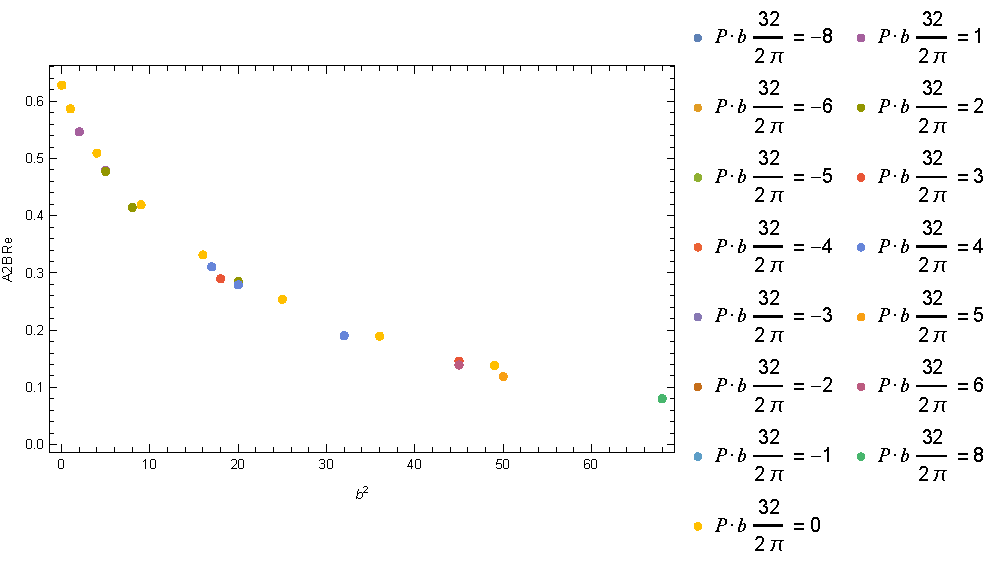
\includegraphics[width=\textwidth]{bsq_A2B_b_even_P1_-1_eta_0.pdf}
     \end{subfigure}
        \caption{Plot of $\tAmp^{\text{Re}}_{2B}=\tAmp^{\text{(b-even)}}_{2B}$ for different Lorentz invariant $P\cdot b$ and $(b)^2$  ($P_{1} = -1$ , $\eta=0$)}
\end{figure}

\subsubsection{$\tAmp^{\text{Im}}_{2B}=\tAmp^{\text{(b-odd)}}_{2B}$}
\begin{figure}[h!]
    \centering
    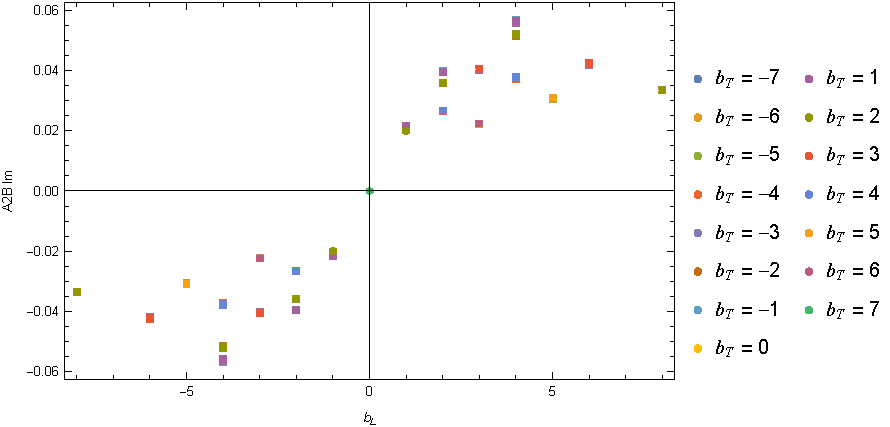
\includegraphics[width=0.45\linewidth]{bLbT_A2B_b_odd_P1_-1_eta_0.pdf}
    \caption{Plot of  $\tAmp^{\text{Im}}_{2B}=\tAmp^{\text{(b-odd)}}_{2B}$ for different $b_{L}$ and $b_{T}$  ($P_{1} = -1$ , $\eta=0$)}
\end{figure}

\pagebreak

And below is the plot of $\tAmp^{\text{Im}}_{2B}=\tAmp^{\text{(b-odd)}}_{2B}$ for different Lorentz invariant $P\cdot b$ and $(b)^2$,
\begin{figure}[h!]
     \centering
     \begin{subfigure}[b]{0.45\textwidth}
         \centering
         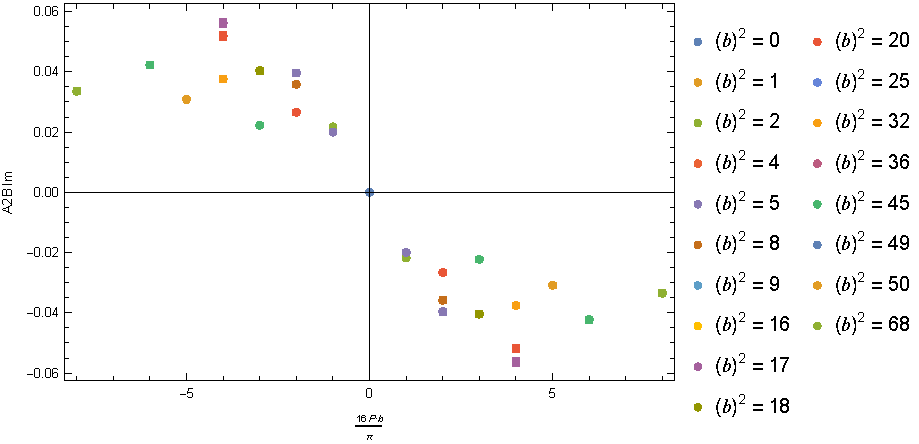
\includegraphics[width=\textwidth]{bP_A2B_b_odd_P1_-1_eta_0.pdf}
     \end{subfigure}
     \begin{subfigure}[b]{0.45\textwidth}
         \centering
         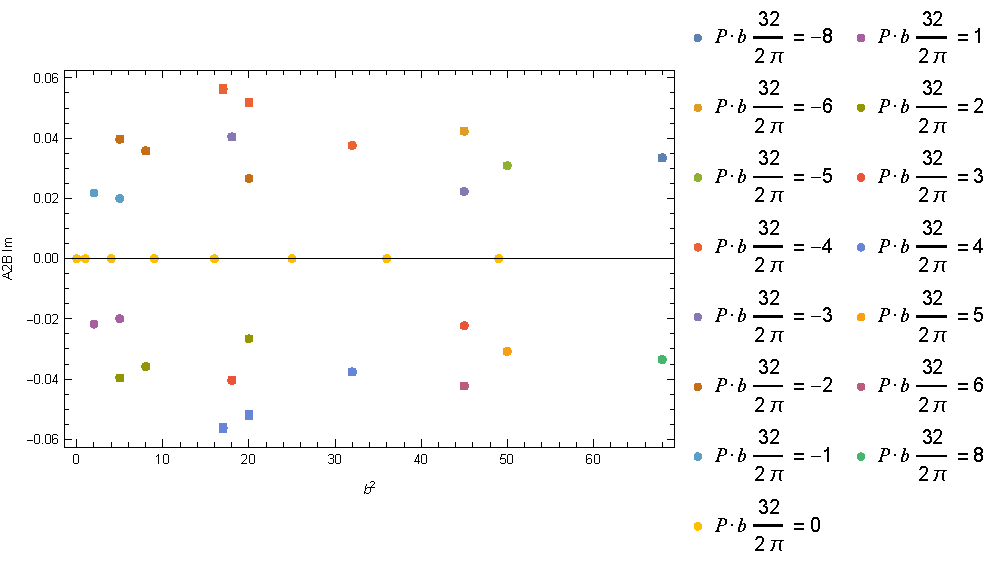
\includegraphics[width=\textwidth]{bsq_A2B_b_odd_P1_-1_eta_0.pdf}
     \end{subfigure}
        \caption{Plot of $\tAmp^{\text{Im}}_{2B}=\tAmp^{\text{(b-odd)}}_{2B}$ for different Lorentz invariant $P\cdot b$ and $(b)^2$  ($P_{1} = -1$ , $\eta=0$)}
\end{figure}



\section{Lattice calculations (new data)}
The lattice setup is $P^{\mu}=(E_N, -|\vec{P}^1|,0,0)$, $b^{\mu}=(0,b_{1},b_{2},0)$, $v^{\mu}=\pm n^{\prime}(0,v_{1},0,v_{3})$, $S^{\mu}=(0,0,0,1)$:
\subsection{Sivers $\tAmp_{12B}$}
\subsubsection{$\tAmp^{\text{Re}}_{12B}=\tAmp^{\text{(b-even)}}_{12B}$}
\begin{figure}[h!]
    \centering
    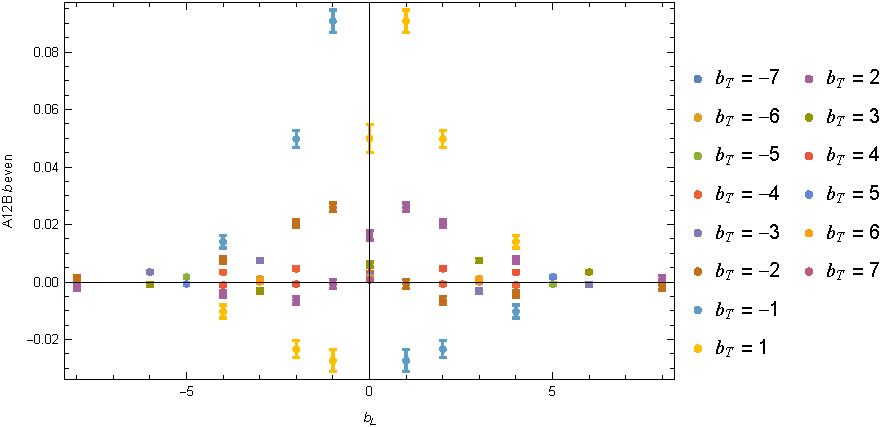
\includegraphics[width=0.45\linewidth]{bLbT_A12B_b_even_P1_-1_eta_8.pdf}
    \caption{Plot of  $\tAmp^{\text{Re}}_{12B}=\tAmp^{\text{(b-even)}}_{12B}$ for different $b_{L}$ and $b_{T}$  ($P_{1} = -1$ , $\eta=8$)}
\end{figure}


Since $\tAmp_{12B}(\bvec^2,\bvec \tcdot P,(\bvec \tcdot P) R(\zetahat^2)/\mN^2,-1/(\mN\zetahat)^2,\eta v \tcdot P)$, below is the plot of $\tAmp^{\text{Re}}_{12B}=\tAmp^{\text{(b-even)}}_{12B}$ for different Lorentz invariant $P\cdot b$ and $(b)^2$,
\begin{figure}[h!]
     \centering
     \begin{subfigure}[b]{0.45\textwidth}
         \centering
         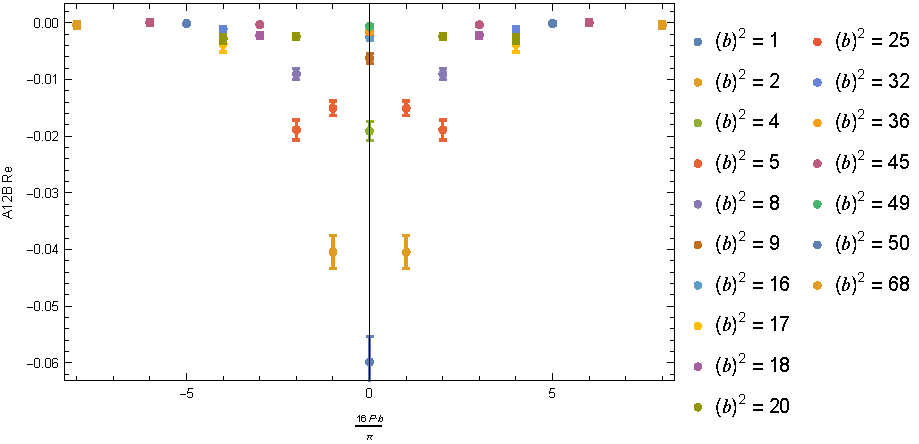
\includegraphics[width=\textwidth]{bP_A12B_b_even_P1_-1_eta_8.pdf}
     \end{subfigure}
     \begin{subfigure}[b]{0.45\textwidth}
         \centering
         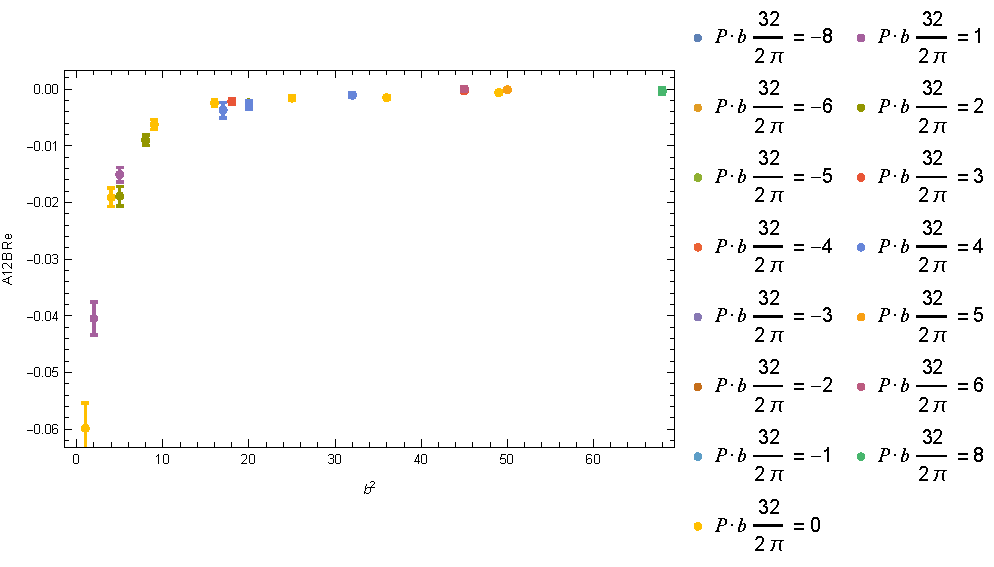
\includegraphics[width=\textwidth]{bsq_A12B_b_even_P1_-1_eta_8.pdf}
     \end{subfigure}
        \caption{Plot of $\tAmp^{\text{Re}}_{12B}=\tAmp^{\text{(b-even)}}_{12B}$ for different Lorentz invariant $P\cdot b$ and $(b)^2$  ($P_{1} = -1$ , $\eta=8$)}
\end{figure}


\subsubsection{$\tAmp^{\text{Im}}_{12B}=\tAmp^{\text{(b-odd)}}_{12B}$}
\begin{figure}[h!]
    \centering
    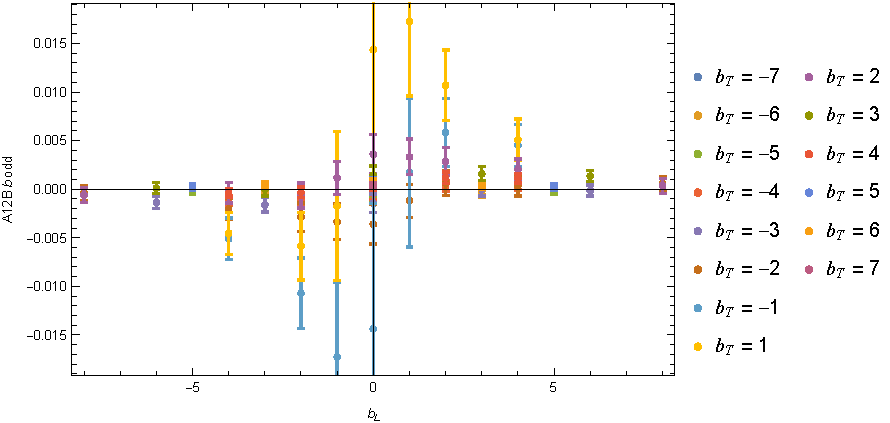
\includegraphics[width=0.45\linewidth]{bLbT_A12B_b_odd_P1_-1_eta_8.pdf}
    \caption{Plot of  $\tAmp^{\text{Im}}_{12B}=\tAmp^{\text{(b-odd)}}_{12B}$ for different $b_{L}$ and $b_{T}$  ($P_{1} = -1$ , $\eta=8$)}
\end{figure}



And below is the plot of $\tAmp^{\text{Im}}_{12B}=\tAmp^{\text{(b-odd)}}_{12B}$ for different Lorentz invariant $P\cdot b$ and $(b)^2$,
\begin{figure}[h!]
     \centering
     \begin{subfigure}[b]{0.45\textwidth}
         \centering
         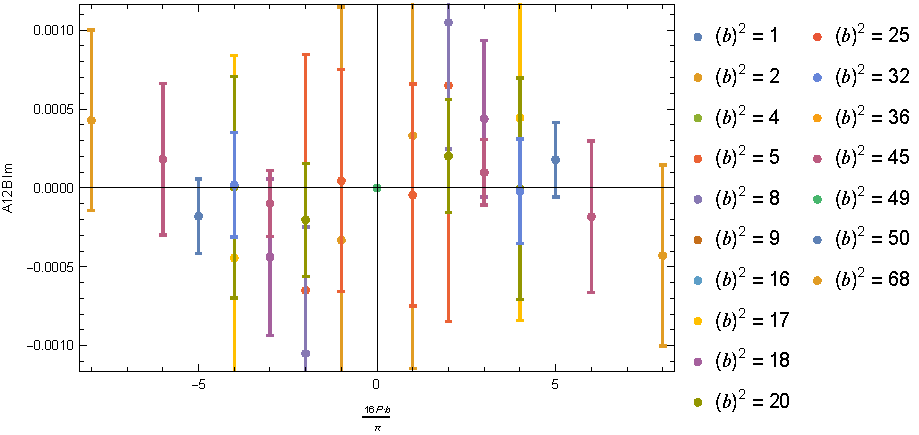
\includegraphics[width=\textwidth]{bP_A12B_b_odd_P1_-1_eta_8.pdf}
     \end{subfigure}
     \begin{subfigure}[b]{0.45\textwidth}
         \centering
         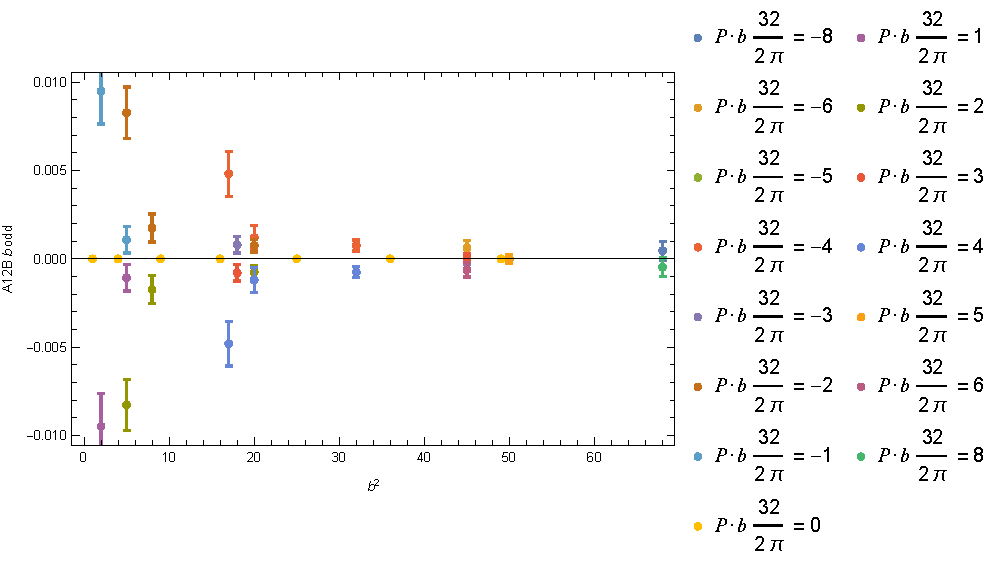
\includegraphics[width=\textwidth]{bsq_A12B_b_odd_P1_-1_eta_8.pdf}
     \end{subfigure}
        \caption{Plot of $\tAmp^{\text{Im}}_{12B}=\tAmp^{\text{(b-odd)}}_{12B}$ for different Lorentz invariant $P\cdot b$ and $(b)^2$  ($P_{1} = -1$ , $\eta=8$)}
\end{figure}





\subsubsection{$\tAmp^{\text{Re}}_{2B}=\tAmp^{\text{(b-even)}}_{2B}$}
\begin{figure}[h!]
    \centering
    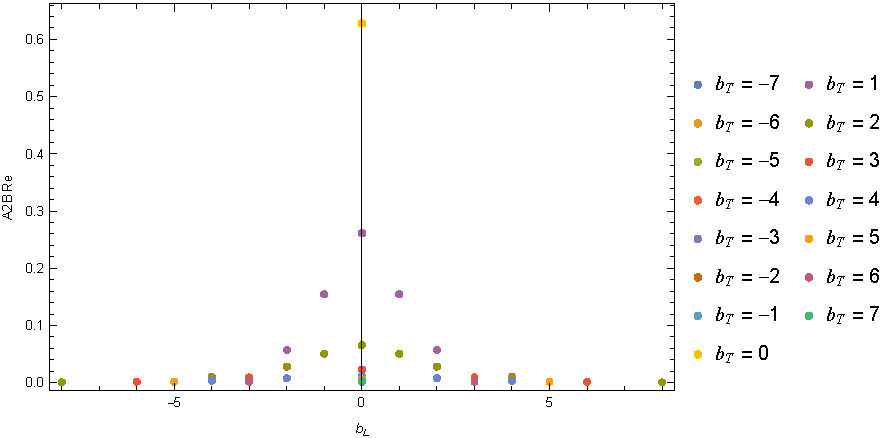
\includegraphics[width=0.45\linewidth]{bLbT_A2B_b_even_P1_-1_eta_8.pdf}
    \caption{Plot of  $\tAmp^{\text{Re}}_{2B}=\tAmp^{\text{(b-even)}}_{2B}$ for different $b_{L}$ and $b_{T}$  ($P_{1} = -1$ , $\eta=8$)}
\end{figure}

And below is the plot of $\tAmp^{\text{Re}}_{2B}=\tAmp^{\text{(b-even)}}_{2B}$ for different Lorentz invariant $P\cdot b$ and $(b)^2$,
\begin{figure}[h!]
     \centering
     \begin{subfigure}[b]{0.45\textwidth}
         \centering
         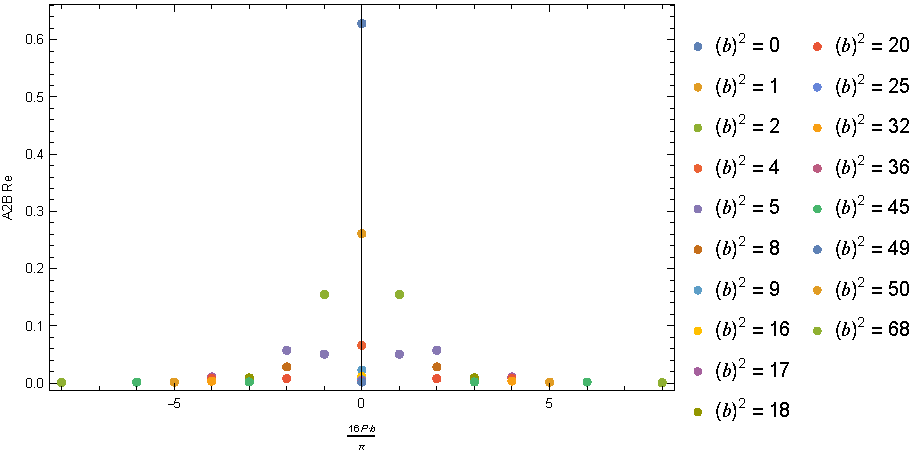
\includegraphics[width=\textwidth]{bP_A2B_b_even_P1_-1_eta_8.pdf}
     \end{subfigure}
     \begin{subfigure}[b]{0.45\textwidth}
         \centering
         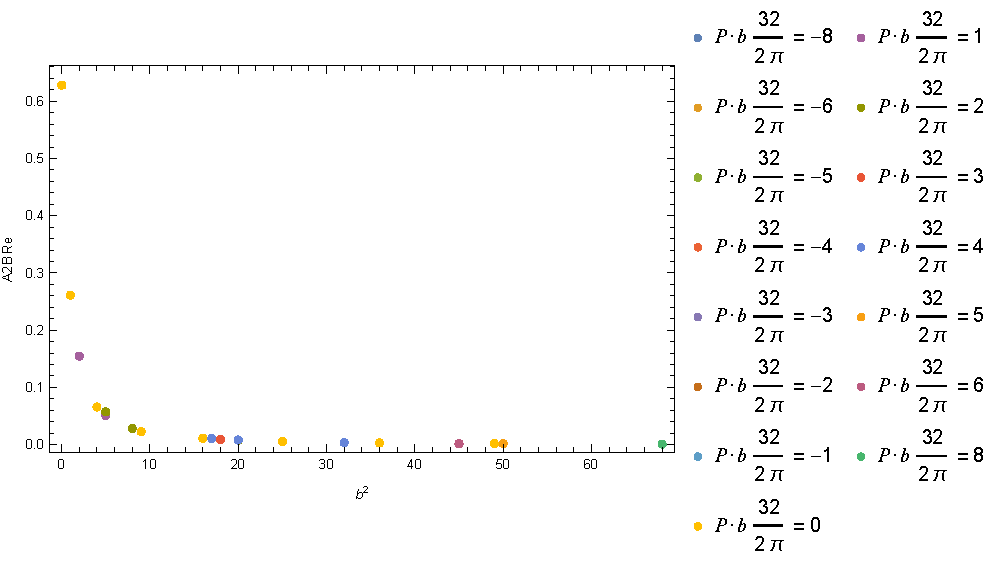
\includegraphics[width=\textwidth]{bsq_A2B_b_even_P1_-1_eta_8.pdf}
     \end{subfigure}
        \caption{Plot of $\tAmp^{\text{Re}}_{2B}=\tAmp^{\text{(b-even)}}_{2B}$ for different Lorentz invariant $P\cdot b$ and $(b)^2$  ($P_{1} = -1$ , $\eta=8$)}
\end{figure}

\subsubsection{$\tAmp^{\text{Im}}_{2B}=\tAmp^{\text{(b-odd)}}_{2B}$}
\begin{figure}[h!]
    \centering
    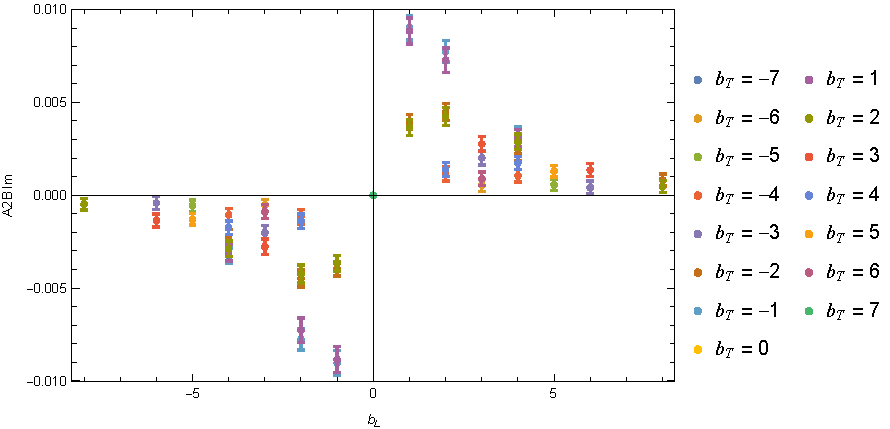
\includegraphics[width=0.45\linewidth]{bLbT_A2B_b_odd_P1_-1_eta_8.pdf}
    \caption{Plot of  $\tAmp^{\text{Im}}_{2B}=\tAmp^{\text{(b-odd)}}_{2B}$ for different $b_{L}$ and $b_{T}$  ($P_{1} = -1$ , $\eta=8$)}
\end{figure}

\pagebreak

And below is the plot of $\tAmp^{\text{Im}}_{2B}=\tAmp^{\text{(b-odd)}}_{2B}$ for different Lorentz invariant $P\cdot b$ and $(b)^2$,
\begin{figure}[h!]
     \centering
     \begin{subfigure}[b]{0.45\textwidth}
         \centering
         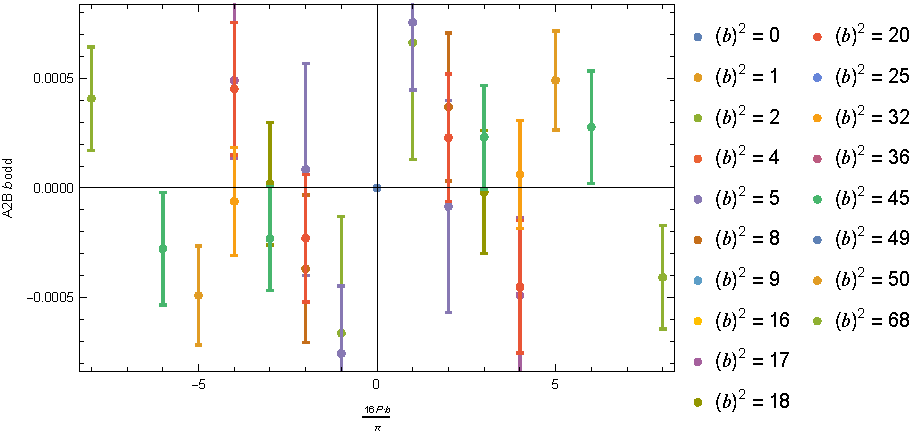
\includegraphics[width=\textwidth]{bP_A2B_b_odd_P1_-1_eta_8.pdf}
     \end{subfigure}
     \begin{subfigure}[b]{0.45\textwidth}
         \centering
         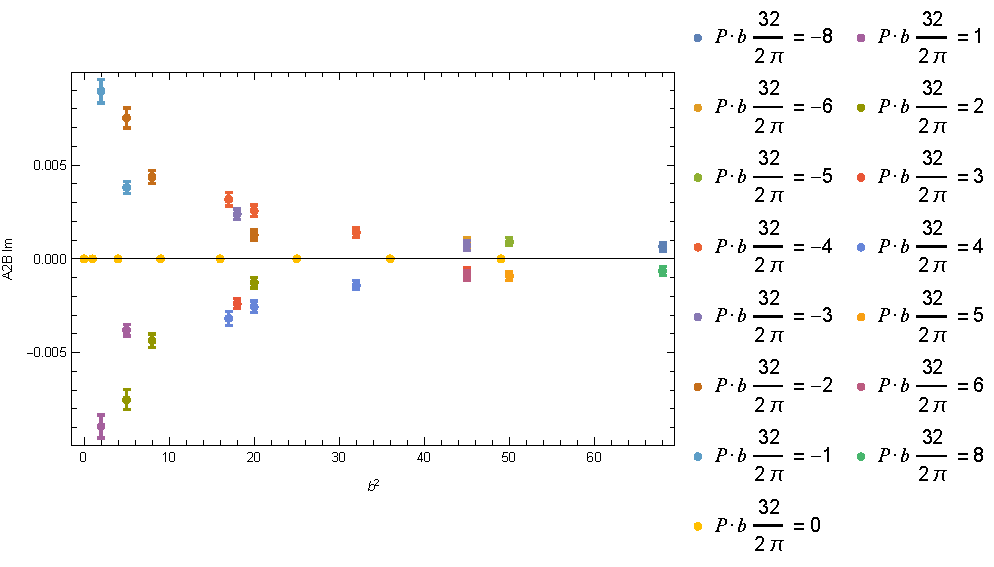
\includegraphics[width=\textwidth]{bsq_A2B_b_odd_P1_-1_eta_8.pdf}
     \end{subfigure}
        \caption{Plot of $\tAmp^{\text{Im}}_{2B}=\tAmp^{\text{(b-odd)}}_{2B}$ for different Lorentz invariant $P\cdot b$ and $(b)^2$  ($P_{1} = -1$ , $\eta=8$)}
\end{figure}




\end{document}